\documentclass[12pt,a4paper,oneside]{report}

% ===== GEOMETRY & TYPOGRAPHY =====
\usepackage[top=1in, bottom=1.0in, right=1in, left=1.25in]{geometry}
\usepackage{mathptmx}
\usepackage{setspace}
\onehalfspacing
\usepackage{titlesec}
\usepackage{graphicx}
\usepackage{booktabs}
\usepackage{tabularx}
\usepackage{longtable}
\usepackage{array}
\usepackage[hidelinks]{hyperref}
\usepackage{fancyhdr}
\usepackage{listings}
\usepackage{enumitem}
\usepackage{amsmath,amssymb}
\usepackage{caption}
\usepackage{subcaption}
\usepackage{float}
\usepackage{xcolor}
\usepackage{tikz}
\usetikzlibrary{shapes.geometric, arrows, positioning, shadows, fit, calc}
\usepackage{multirow}
\usepackage{appendix}
\usepackage{pdfpages}

% ===== SPACING & LAYOUT CONTROLS (Tuned for ~65 Pages Target) =====
\setlength{\parindent}{0pt}
\setlength{\parskip}{0.5em}
\setlength{\textfloatsep}{12pt plus 2pt minus 2pt}
\setlength{\intextsep}{12pt plus 2pt minus 2pt}
\raggedbottom
\widowpenalty=10000
\clubpenalty=10000

% ===== ELEGANT CENTERED CHAPTER TITLE PAGE COMMAND =====
\newcommand{\makechaptertitlepage}[2]{%
  \cleardoublepage
  \thispagestyle{empty}
  \vspace*{\fill}
  \begin{center}
    {\Large \scshape \bfseries \color{blue!85!black} CHAPTER #1}\\[0.2in]
    {\color{gray!40}\rule{3.8in}{1.2pt}}\\[0.3in]
    {\Huge \bfseries \color{black} #2}\\[0.3in]
    {\color{gray!40}\rule{3.8in}{1.2pt}}
  \end{center}
  \vspace*{\fill}
  \newpage
}

% ===== SCREENSHOT PLACEHOLDER (OPTIMIZED HALF PAGE CONTAINER) =====
\newcommand{\screenshotplaceholder}[1]{%
  \begin{figure}[htbp]
  \centering
  \fbox{\begin{minipage}[c][3.0in][c]{0.92\textwidth}
    \centering
    \vfill
    {\Large \bfseries SCREENSHOT PLACEHOLDER}\\[0.15in]
    {\large \itshape (Insert actual screenshot here)}\\[0.2in]
    {\textbf{#1}}
    \vfill
  \end{minipage}}
  \caption{#1}
  \end{figure}
}

% ===== CHAPTER FORMAT (suppress "Chapter X" on text pages) =====
\titleformat{\chapter}[display]
  {\normalfont\Huge\bfseries\centering}{}{0pt}{}
\titlespacing*{\chapter}{0pt}{-20pt}{18pt}

\titleformat{\section}{\normalfont\Large\bfseries}{\thesection}{1em}{}
\titleformat{\subsection}{\normalfont\large\bfseries}{\thesubsection}{1em}{}
\titleformat{\subsubsection}{\normalfont\normalsize\bfseries}{\thesubsubsection}{1em}{}

% ===== CODE LISTINGS =====
\lstset{
  basicstyle=\ttfamily\footnotesize,
  breaklines=true,
  frame=single,
  numbers=left,
  numberstyle=\tiny\color{gray},
  keywordstyle=\bfseries\color{blue!70!black},
  commentstyle=\itshape\color{green!50!black},
  stringstyle=\color{red!60!black},
  showstringspaces=false,
  tabsize=2,
  xleftmargin=1.5em,
  framexleftmargin=1.5em,
  captionpos=b
}

% ===== HEADERS & FOOTERS =====
\pagestyle{fancy}
\fancyhf{}
% Header: Left = SMARTHIRE : Hiring Solutions, Right = 2026
\lhead{\small\scshape SMARTHIRE : Hiring Solutions}
\rhead{\small\scshape 2026}

% Footer: Left = Department of CSE, North Campus, University of Kashmir, Right = Page Number
\lfoot{\small\scshape Department of CSE, North Campus, University of Kashmir}
\rfoot{\thepage}

\renewcommand{\headrulewidth}{0.4pt}
\renewcommand{\footrulewidth}{0.4pt}

% ===================================================================
\begin{document}

% --- Frontmatter ---
\begin{titlepage}
    \centering
    \vspace*{0.3in}

    {\Huge \bfseries SMARTHIRE}\\[0.25in]
    {\Large \bfseries AN AUTONOMOUS MULTI-STAGE RECRUITMENT AND CANDIDATE EVALUATION PLATFORM}\\[0.4in]

    \textit{A Major Project Report Submitted in Partial Fulfillment of the\\Requirements for the Award of the Degree of}\\[0.2in]

    {\Large \bfseries Bachelor of Technology}\\[0.05in]
    {\large \bfseries in}\\[0.05in]
    {\Large \bfseries Computer Science and Engineering}\\[0.35in]

    \textbf{Submitted By:}\\[0.1in]
    \begin{tabular}{ll}
      \textbf{MIR SUHAIB}        & (Enrollment No: 22048112049) \\
      \textbf{MIR MUSAIB}        & (Enrollment No: 22048112050) \\
      \textbf{FURKAN MUSHTAQ}    & (Enrollment No: 22048112032) \\
      \textbf{KHALID BIN BASHIR} & (Enrollment No: 19048112001) \\
    \end{tabular}\\[0.3in]

    \textbf{Under the Supervision of:}\\[0.08in]
    {\large \textbf{Er.\ Khalid Hussain}}\\[0.04in]
    Assistant Professor\\[0.3in]

    \vfill

    \IfFileExists{images/logo.png}{
\includegraphics[width=0.20\textwidth]{images/logo.png}\\[0.15in]}{}

    {\Large\bfseries
    DEPARTMENT OF COMPUTER SCIENCE AND ENGINEERING\\
    NORTH CAMPUS, UNIVERSITY OF KASHMIR\\
    DELINA, BARAMULLA --- 193103, J\&K\\[0.08in]
    2025 --- 2026
    }
\end{titlepage}
\cleardoublepage

\begin{center}
    {\Large \bfseries DEPARTMENT OF COMPUTER SCIENCE AND ENGINEERING}\\
    {\large \bfseries NORTH CAMPUS, UNIVERSITY OF KASHMIR}\\
    {\large \bfseries DELINA, BARAMULLA --- 193103, J\&K}\\[0.3in]

    \IfFileExists{images/logo.png}{
\includegraphics[width=0.18\textwidth]{images/logo.png}\\[0.2in]}{}

    {\null \Large \bfseries CERTIFICATE}\\[0.2in]
\end{center}

This is to certify that the project work entitled \textbf{``SMARTHIRE: AN AUTONOMOUS MULTI-STAGE RECRUITMENT AND CANDIDATE EVALUATION PLATFORM''} is a bonafide record of major project work carried out by \textbf{Mir Suhaib (22048112049)}, \textbf{Mir Musaib (22048112050)}, \textbf{Furkan Mushtaq (22048112032)}, and \textbf{Khalid Bin Bashir (19048112001)} under my supervision and guidance in partial fulfillment of the requirements for the award of the degree of \textbf{Bachelor of Technology in Computer Science and Engineering} from the Department of Computer Science \& Engineering, North Campus, University of Kashmir, Delina, Baramulla during the academic session 2025--2026.

\vspace{1.2in}

\begin{table}[H]
\centering
\begin{tabular}{p{2.8in}p{2.8in}}
\textbf{Supervisor:} & \textbf{Coordinator:}\\[0.4in]
\rule{2.4in}{0.4pt} & \rule{2.4in}{0.4pt}\\
\textbf{Er.\ Khalid Hussain} & \textbf{Dr.\ Waseem Jeelani Bakshi}\\
Assistant Professor & Coordinator, Dept.\ of CSE\\
Dept.\ of CSE, North Campus, KU & North Campus, KU, Delina, Baramulla\\
\end{tabular}
\end{table}
\cleardoublepage

\begin{center}
    {\null \Large \bfseries DECLARATION}\\[0.3in]
\end{center}

We hereby declare that the work presented in this major project report entitled \textbf{``SMARTHIRE: AN AUTONOMOUS MULTI-STAGE RECRUITMENT AND CANDIDATE EVALUATION PLATFORM''} submitted to the Department of Computer Science and Engineering, North Campus, University of Kashmir, Delina, Baramulla, is an authentic record of our own research and software development carried out under the guidance of \textbf{Er.\ Khalid Hussain}.

We further declare that the matter embodied in this report has not been submitted by us for the award of any other degree or diploma to any other University or Institute.

\vspace{1.0in}

\begin{tabular}{p{3.2in}l}
\textbf{Mir Suhaib} & (22048112049) \ \ \rule{1.8in}{0.4pt}\\[0.25in]
\textbf{Mir Musaib} & (22048112050) \ \ \rule{1.8in}{0.4pt}\\[0.25in]
\textbf{Furkan Mushtaq} & (22048112032) \ \ \rule{1.8in}{0.4pt}\\[0.25in]
\textbf{Khalid Bin Bashir} & (19048112001) \ \ \rule{1.8in}{0.4pt}\\
\end{tabular}

\vspace{0.4in}
\textbf{Date:} July 24, 2026\\
\textbf{Place:} Delina, Baramulla, J\&K, India
\cleardoublepage

\begin{center}
    {\Large \bfseries ACKNOWLEDGEMENTS}\\[0.25in]
\end{center}

We would like to express our sincere gratitude to our project supervisor, \textbf{Er.\ Khalid Hussain}, Assistant Professor, Department of Computer Science and Engineering, North Campus, University of Kashmir, Delina, Baramulla, for his invaluable guidance, mentorship, and constructive feedback throughout every phase of this project. His technical expertise and patient supervision were instrumental in shaping the architecture and implementation of SmartHire.

We are deeply grateful to \textbf{Dr.\ Waseem Jeelani Bakshi}, Coordinator, Department of Computer Science and Engineering, North Campus, University of Kashmir, for providing the necessary institutional support, laboratory infrastructure, and an encouraging academic environment. We also extend our thanks to all faculty members and technical staff of the department whose teaching and support over the course of our programme laid the foundation for this work.

We acknowledge the open-source communities behind Next.js, Supabase, React, and the Monaco Editor project, whose well-documented tools and libraries made rapid prototyping feasible. The availability of Google's Gemini AI API for research purposes was equally critical to the AI-driven evaluation modules of this platform.

Finally, we owe a debt of gratitude to our families and friends for their unwavering encouragement and patience throughout our undergraduate studies.

\vspace{0.3in}
\begin{flushright}
\textbf{Mir Suhaib}\\
\textbf{Mir Musaib}\\
\textbf{Furkan Mushtaq}\\
\textbf{Khalid Bin Bashir}\\[0.15in]
Delina, Baramulla\\
July 2026
\end{flushright}
\cleardoublepage

\begin{center}
    {\Large \bfseries ABSTRACT}\\[0.25in]
\end{center}

The recruitment industry has undergone significant transformation with the adoption of digital tools, yet the majority of technical hiring workflows remain fragmented across multiple disconnected platforms. Recruiters typically rely on one tool for tracking applicants, another for conducting coding assessments, a third for scheduling and conducting video interviews, and manual processes for generating offer letters. This fragmentation introduces delays, increases administrative overhead, and leaves candidates without clear feedback on their evaluation status.

This report presents \textbf{SmartHire}, a web-based platform that consolidates the entire technical recruitment pipeline into a single application. Built with Next.js~15 on the frontend and Supabase PostgreSQL on the backend, SmartHire provides six core capabilities: automated resume parsing with ATS relevance scoring, timed multiple-choice assessments, an interactive browser-based coding environment powered by the Monaco editor, AI-driven video interview evaluation using Google's Gemini API, a recruiter-facing Kanban pipeline board for managing candidate progression, and automated PDF offer letter generation.

The system employs a multi-schema PostgreSQL architecture to enforce strict data isolation between recruiting organisations. Candidates progress through a sequential evaluation pipeline where each stage produces quantitative scores, and stage-specific rejection tracking ensures that applicants receive transparent feedback. Empirical evaluation with simulated hiring workflows demonstrated a reduction in average screening time from approximately fifteen minutes per candidate to under three seconds for automated stages, while maintaining consistent scoring across repeated evaluations.

\textbf{Keywords:} Applicant Tracking System, Recruitment Automation, Resume Parsing, Code Assessment, AI Video Interview, Multi-Tenant Architecture, Next.js, Supabase PostgreSQL
\cleardoublepage


\cleardoublepage
\pagenumbering{roman}
\tableofcontents
\listoffigures
\listoftables
\chapter*{List of Abbreviations}
\addcontentsline{toc}{chapter}{List of Abbreviations}

\begin{longtable}{p{1.5in}p{4.5in}}
\textbf{Abbreviation} & \textbf{Full Form}\\
\midrule
\endfirsthead
\textbf{Abbreviation} & \textbf{Full Form}\\
\midrule
\endhead
AI    & Artificial Intelligence\\
API   & Application Programming Interface\\
ATS   & Applicant Tracking System\\
CSS   & Cascading Style Sheets\\
CRUD  & Create, Read, Update, Delete\\
DFD   & Data Flow Diagram\\
DOM   & Document Object Model\\
ER    & Entity--Relationship\\
HTML  & HyperText Markup Language\\
HTTP  & HyperText Transfer Protocol\\
IDE   & Integrated Development Environment\\
IEEE  & Institute of Electrical and Electronics Engineers\\
JSON  & JavaScript Object Notation\\
JWT   & JSON Web Token\\
LLM   & Large Language Model\\
MCQ   & Multiple Choice Question\\
NLP   & Natural Language Processing\\
ORM   & Object--Relational Mapping\\
PDF   & Portable Document Format\\
REST  & Representational State Transfer\\
RLS   & Row-Level Security\\
SaaS  & Software as a Service\\
SDK   & Software Development Kit\\
SQL   & Structured Query Language\\
SSR   & Server-Side Rendering\\
TF-IDF & Term Frequency--Inverse Document Frequency\\
UI    & User Interface\\
URL   & Uniform Resource Locator\\
UX    & User Experience\\
\end{longtable}
\cleardoublepage


\cleardoublepage
\pagenumbering{arabic}

% --- Chapters ---
\makechaptertitlepage{1}{INTRODUCTION}
\setcounter{chapter}{0}
\chapter{Introduction}
\label{ch:intro}

\section{Background}
\label{sec:background}

The process of identifying, evaluating, and hiring qualified personnel has always been central to organisational success. In the software industry, where technical competence directly determines product quality, the stakes are particularly high. A single poor hiring decision can cost an organisation between fifty and two hundred percent of the employee's annual salary when accounting for onboarding, training, lost productivity, and eventual replacement~\cite{shrm2022}. Despite these high stakes, the tools and methods used by most recruiting teams have not kept pace with the complexity of modern technical roles.

A typical technical hiring workflow involves several sequential stages: sourcing candidates, screening resumes, administering written or online assessments, conducting technical interviews, evaluating cultural fit, and extending offers. Each of these stages has traditionally been handled by a different tool or manual process. Resume screening is done by hand or through basic keyword-matching systems. Coding assessments are administered on third-party platforms such as HackerRank or Codility, which operate independently of the company's applicant tracking system. Video interviews are conducted over general-purpose conferencing tools, with evaluators recording scores on spreadsheets. Offer letters are drafted manually in word processors and sent via email.

This fragmentation creates a range of operational problems. Candidate data is scattered across multiple platforms, making it difficult to construct a unified view of each applicant's progress. Scores from different stages must be manually aggregated, introducing transcription errors and delays. Candidates frequently receive no feedback when they are rejected, leaving them uncertain about where their application fell short. Recruiters spend a disproportionate amount of time on administrative coordination rather than substantive evaluation.

\section{Evolution of Recruitment Technology}
\label{sec:evolution}

Recruitment technology has evolved through several distinct phases, each driven by broader trends in computing and connectivity.

\subsection{Manual and Paper-Based Systems (Pre-2000)}

Before the widespread adoption of the internet, recruitment was an entirely manual affair. Job vacancies were advertised in newspapers, trade journals, and university placement offices. Applications arrived as physical documents---printed resumes accompanied by cover letters---which were filed in cabinets and reviewed by hand. Shortlisting decisions were based on a recruiter's subjective reading of each resume, with no standardised scoring. Interview scheduling involved telephone calls and physical appointment books. The entire process, from posting a vacancy to extending an offer, routinely took sixty to ninety days~\cite{cappelli2019}.

\subsection{Early Digital Systems (2000--2010)}

The first generation of Applicant Tracking Systems emerged in the early 2000s, driven by the growth of online job boards such as Monster.com and Naukri.com. These systems digitised the resume collection process: candidates submitted applications through web forms, and recruiters could search stored resumes using keyword queries. However, these early ATS platforms were essentially databases with search functionality. They did not evaluate candidates; they merely stored and retrieved documents. Screening remained a manual activity, and assessment, interviewing, and offer management continued to rely on separate tools~\cite{cappelli2019}.

\subsection{Cloud-Based Recruitment Platforms (2010--2020)}

The second generation brought cloud-hosted platforms such as Greenhouse, Lever, and Workday Recruiting. These systems introduced structured hiring workflows, collaborative evaluation features, and integration with third-party tools via APIs. Recruiters could define custom pipeline stages, attach interview scorecards, and generate basic analytics. Simultaneously, specialised assessment platforms like HackerRank and Codility emerged to address the growing demand for objective technical evaluation. Video interviewing platforms such as HireVue began using structured question formats and, later, rudimentary AI-based sentiment analysis~\cite{hmoud2020}.

Despite these advances, the fundamental problem of fragmentation persisted. A recruiting team using Greenhouse for tracking, HackerRank for coding tests, and Zoom for interviews still needed to manually transfer data between systems. Each additional tool increased the total cost of ownership and the risk of data inconsistency.

\subsection{AI-Augmented Recruitment (2020--Present)}

The current generation of recruitment technology leverages advances in natural language processing, large language models, and computer vision. Resume parsing engines can now extract structured data from unstructured PDF documents with high accuracy. AI models can score candidate--job fit based on semantic similarity rather than simple keyword overlap. Automated coding sandboxes execute candidate submissions against predefined test suites, producing objective performance metrics. Video interview platforms analyse speech patterns, response coherence, and communication clarity using multimodal AI models~\cite{black2020}.

SmartHire belongs to this latest generation but distinguishes itself by integrating all of these capabilities---ATS tracking, resume scoring, MCQ assessment, coding evaluation, AI video analysis, and offer management---into a single, cohesive platform.

\section{Problems with Existing Technical Hiring Practices}
\label{sec:problems}

Several specific problems motivate the development of SmartHire.

\textbf{Prolonged hiring cycles.} Industry surveys report that the average time to fill a software engineering position ranges from forty-two to sixty-eight days~\cite{shrm2022}. Much of this duration is consumed by administrative tasks: coordinating between platforms, aggregating scores, scheduling interviews, and drafting offer letters. Automated systems can compress these steps from hours to seconds.

\textbf{Inconsistent evaluation standards.} When different recruiters screen resumes for the same role, they often arrive at different shortlists. Research by Kuncel et al.\ demonstrated that unstructured evaluations exhibit low inter-rater reliability, meaning that the outcome depends as much on the evaluator as on the candidate~\cite{kuncel2013}. Automated scoring eliminates this variability for the structured stages of evaluation.

\textbf{Lack of candidate transparency.} Most recruitment systems treat the candidate as a passive participant. Applications are submitted into a void, and rejection notifications---when they arrive at all---provide no actionable information. A system that tracks candidates through well-defined stages and communicates the specific stage at which they were rejected offers a materially better candidate experience.

\textbf{High tooling costs.} An enterprise that subscribes to separate services for applicant tracking, coding assessment, video interviewing, and offer management may spend tens of thousands of dollars annually on software licences alone. A unified platform reduces this to a single subscription or deployment cost.

\textbf{Data isolation failures.} Multi-tenant recruitment platforms must ensure that one organisation's candidate data is never visible to another. Achieving this with application-level access controls is error-prone; schema-level isolation in the database provides a stronger guarantee~\cite{postgresql2024}.

\section{Motivation}
\label{sec:motivation}

The motivation for SmartHire arose from direct observation of these problems during internship experiences and campus placement processes. We observed that even well-resourced recruiting teams spent a substantial fraction of their time on mechanical tasks---copying scores from one platform into another, chasing candidates for scheduling confirmations, and reformatting offer letters---rather than on the qualitative judgements that genuinely require human expertise.

We hypothesised that a platform which automated the mechanical stages of recruitment while preserving human decision-making authority at critical junctures (such as final hiring decisions) would deliver three benefits: faster hiring cycles, more consistent candidate evaluation, and a superior experience for applicants. SmartHire was designed and built to test this hypothesis.

\section{Problem Statement}
\label{sec:problem-statement}

\textit{Design and implement a web-based recruitment platform that integrates applicant tracking, automated resume scoring, timed assessments, browser-based code execution, AI-driven video interview evaluation, and offer letter generation into a unified multi-tenant system, with the goal of reducing manual effort in technical hiring while maintaining evaluation objectivity and candidate transparency.}

\section{Objectives}
\label{sec:objectives}

The project pursued the following specific objectives:

\begin{enumerate}[label=\textbf{O\arabic*.}, leftmargin=1.8em]
  \item Design a multi-schema PostgreSQL database architecture that isolates data across recruiting organisations while supporting efficient cross-schema queries for platform-wide analytics.
  \item Implement an automated resume parsing and ATS scoring module that extracts structured candidate data from PDF uploads and computes a relevance score against job requirements on a zero-to-ten scale.
  \item Build a timed MCQ assessment engine with configurable question pools, randomised question ordering, automatic timer enforcement, and instant score computation.
  \item Develop an interactive, browser-based coding assessment environment using the Monaco editor, supporting multiple programming languages with automated test case execution and grading.
  \item Integrate an AI-powered video interview module that presents structured questions, records candidate responses, and generates evaluation scorecards using Google's Gemini API.
  \item Construct a recruiter-facing Kanban pipeline board that visualises candidate progression across hiring stages and supports drag-and-drop stage transitions with real-time database synchronisation.
  \item Implement automated PDF offer letter generation with customisable templates, digital signature placeholders, and email dispatch.
  \item Validate the platform through systematic testing, including unit tests, integration tests, and simulated end-to-end hiring workflows.
\end{enumerate}

\section{Scope and Contributions}
\label{sec:scope}

SmartHire encompasses two primary user-facing portals and a set of backend services:

\textbf{Candidate Portal.} Candidates can browse published job listings, submit applications with resume uploads, complete timed MCQ assessments, solve coding challenges in a browser-based IDE, participate in AI video interviews, track their application status across stages, and accept or decline offer letters.

\textbf{Recruiter Portal.} Recruiters can create and manage job postings, review parsed resumes and ATS scores, manage candidate pipelines through a Kanban board, schedule interviews, review AI-generated evaluation scorecards, and generate and dispatch offer letters.

\textbf{Backend Services.} The platform's backend provides RESTful API endpoints for authentication, job management, application processing, assessment administration, interview scheduling, and analytics. Data is stored in Supabase PostgreSQL with schema-level multi-tenancy.

The following are explicitly outside the scope of this project: mobile native applications, real-time collaborative editing of job descriptions, integration with external calendar systems (Google Calendar, Outlook), and support for non-technical hiring workflows.

\section{Organisation of the Report}
\label{sec:organisation}

The remainder of this report is structured as follows:

\begin{itemize}[leftmargin=1.5em]
  \item \textbf{Chapter~2} surveys existing literature on recruitment automation, resume parsing, AI-based interview systems, and online code assessment platforms, and identifies the research gaps that SmartHire addresses.
  \item \textbf{Chapter~3} specifies the functional and non-functional requirements, defines the system's actors and use cases, details the technology stack, and presents a feasibility analysis.
  \item \textbf{Chapter~4} describes the system's architecture through multiple perspectives: high-level architecture, database schema design, data flow diagrams, sequence diagrams, and workflow specifications for each major subsystem.
  \item \textbf{Chapter~5} provides an in-depth account of the implementation of each module, including code excerpts, design decisions, and integration patterns.
  \item \textbf{Chapter~6} documents the testing strategy and presents detailed test cases spanning unit, integration, system, performance, and security testing.
  \item \textbf{Chapter~7} reports empirical results, discusses performance metrics, and analyses the strengths and limitations of the implemented system.
  \item \textbf{Chapter~8} concludes the report with a summary of contributions, a discussion of limitations, and directions for future work.
\end{itemize}


\makechaptertitlepage{2}{LITERATURE SURVEY}
\setcounter{chapter}{1}
\chapter{Literature Survey}
\label{ch:litsurvey}

\section{Overview}
\label{sec:lit-intro}

This chapter surveys academic literature and enterprise platforms across four domain areas: applicant tracking pipelines, resume parsing systems, technical assessment platforms, and AI video interview evaluators.

\section{Review of Commercial Systems}
\label{sec:ats-review}

Commercial ATS platforms such as Greenhouse~\cite{greenhouse2024}, Lever~\cite{lever2024}, and Workday~\cite{workday2024} provide structured hiring pipelines and collaborative scoring. However, these systems operate purely as workflow tools and do not natively evaluate technical candidate skills. External coding platforms (HackerRank, Codility) and video tools (HireVue) require custom API integrations, introducing data synchronization overhead and increasing recruiter workload by 20--30\%~\cite{nguyen2021}.

\section{Resume Parsing and Vector Similarity Scoring}
\label{sec:resume-review}

Early resume parsers relied on regular expressions and rule-based templates, which struggled with non-standard formatting~\cite{yu2005}. Machine learning models introduced named entity recognition (NER) for skill extraction~\cite{jiechieu2021}. Modern systems vectorise resumes and job descriptions into high-dimensional embedding spaces, computing match relevance via cosine similarity:
\begin{equation}
\label{eq:cosine}
\text{sim}(\vec{r}, \vec{j}) = \frac{\vec{r} \cdot \vec{j}}{\|\vec{r}\| \cdot \|\vec{j}\|}
\end{equation}
SmartHire builds on this by leveraging Google's Gemini API to calculate multi-dimensional relevance scores (0--10 scale).

\section{Technical Assessments and AI Interviewing}
\label{sec:assessment-review}

Coding assessment platforms like HackerRank~\cite{hackerrank2024} and Codility~\cite{codility2024} provide sandboxed code execution but operate in isolation from ATS candidate boards. In video interviewing, HireVue pioneered AI-assisted candidate evaluation~\cite{hirevue2024}. Academic studies demonstrate that multimodal LLMs effectively evaluate candidate response depth and technical clarity as decision-support tools~\cite{chen2022, naim2018}.

\section{Multi-Tenant Database Architectures}
\label{sec:multitenancy-review}

Multi-tenant SaaS platforms enforce data isolation through separate databases, shared database with separate schemas, or shared schemas with tenant IDs~\cite{chong2006}. SmartHire adopts domain-specific schemas (\texttt{organization}, \texttt{job}, \texttt{candidate}, \texttt{application}, \texttt{assessment}, \texttt{interview}) with PostgreSQL Row-Level Security (RLS) for complete multi-tenant isolation~\cite{supabase2024}.

\section{Comparative Analysis}
\label{sec:comparison}

\begin{table}[htbp]
\centering
\caption{Feature comparison of existing systems vs. SmartHire}
\label{tab:comparison}
\small
\begin{tabular}{lccccc}
\toprule
\textbf{Capability} & \textbf{Greenhouse} & \textbf{HackerRank} & \textbf{HireVue} & \textbf{TestGorilla} & \textbf{SmartHire} \\
\midrule
ATS Pipeline Tracking          & \checkmark & ---        & ---        & ---        & \checkmark \\
Automated Resume Scoring       & Partial    & ---        & ---        & ---        & \checkmark \\
Timed MCQ Assessments          & ---        & \checkmark & ---        & \checkmark & \checkmark \\
Browser Code Execution IDE     & ---        & \checkmark & ---        & ---        & \checkmark \\
AI Video Interview Auditing    & ---        & ---        & \checkmark & ---        & \checkmark \\
Stage Rejection Feedback       & Partial    & ---        & ---        & ---        & \checkmark \\
Automated PDF Offer Generator   & \checkmark & ---        & ---        & ---        & \checkmark \\
Unified Single-Platform SaaS   & ---        & ---        & ---        & ---        & \checkmark \\
\bottomrule
\end{tabular}
\end{table}

\section{Research Gap Identification}
\label{sec:research-gap}

Existing platforms leave three principal gaps: (1) Fragmented toolchains requiring manual score transfers across vendor portals; (2) Lack of transparent rejection feedback informing candidates of their specific disqualification stage; and (3) High subscription cost for licensing multiple standalone tools. SmartHire fills these gaps within a single SaaS ecosystem.


\makechaptertitlepage{3}{REQUIREMENT ANALYSIS}
\setcounter{chapter}{2}
\chapter{Requirement Analysis}
\label{ch:requirements}

\section{Overview}
\label{sec:req-overview}

This chapter specifies the requirements that guided the design and implementation of SmartHire. Requirements are organised into functional requirements (what the system must do), non-functional requirements (how well it must do it), and operational constraints. We also present a feasibility study, define the system's actors and use cases, detail the technology stack, and discuss risk factors.

\section{System Actors}
\label{sec:actors}

SmartHire supports three categories of users, each with distinct permissions and workflows:

\begin{enumerate}[leftmargin=1.5em]
  \item \textbf{Candidate}: An individual seeking employment who registers on the platform, browses job listings, submits applications, completes assessments, participates in interviews, and tracks application status.
  \item \textbf{Recruiter}: An employee of a hiring organisation who creates job postings, reviews candidate applications and scores, manages the hiring pipeline, schedules interviews, and generates offer letters. Each recruiter is associated with exactly one company.
  \item \textbf{Administrator}: A platform operator with access to system-wide analytics, user management, and configuration settings.
\end{enumerate}

\section{Functional Requirements}
\label{sec:functional-reqs}

\subsection{Candidate Portal Requirements}

The Candidate Portal serves as the primary interface for job seekers using the platform. Candidates require an intuitive, frictionless experience that allows them to discover opportunities, present their credentials, complete technical evaluations, and track their progress transparently across all hiring stages.

Key functional capabilities of the candidate portal include account registration, profile management, searchable job directory browsing, resume upload with automated text extraction, multi-stage assessment participation (timed MCQs, interactive browser-based coding, and AI video interviews), real-time application tracking with explicit stage-by-stage status feedback, and offer letter review. Table~\ref{tab:fr-candidate} summarizes the specific functional requirement statements for the Candidate Portal.

\begin{table}[htbp]
\centering
\caption{Functional requirements: Candidate Portal}
\label{tab:fr-candidate}
\small
\begin{tabular}{p{0.8in}p{4.8in}}
\toprule
\textbf{ID} & \textbf{Description} \\
\midrule
FR-C01 & The system shall allow candidates to register using email and password credentials, with email verification. \\
FR-C02 & The system shall allow candidates to create and edit a profile containing personal information, skills, education, and work experience. \\
FR-C03 & The system shall display a searchable, filterable directory of published job listings. Filters shall include job category, location, employment type, and keyword search. \\
FR-C04 & The system shall allow candidates to apply for a job by uploading a PDF resume. The resume shall be parsed automatically to extract structured candidate data. \\
FR-C05 & The system shall compute an ATS relevance score (0--10) for each application by comparing the parsed resume against the job's required skills and qualifications. \\
FR-C06 & The system shall present timed MCQ assessments to candidates who advance past the ATS screening stage. Assessments shall enforce a countdown timer and auto-submit upon expiry. \\
FR-C07 & The system shall provide a browser-based coding environment (Monaco editor) for candidates to solve coding challenges, with real-time test case execution and automated scoring. \\
FR-C08 & The system shall provide an AI video interview interface that presents structured questions, records candidate responses, and submits them for AI evaluation. \\
FR-C09 & The system shall display a candidate's application history showing the current stage, scores at each completed stage, and, for rejected applications, the specific stage of rejection. \\
FR-C10 & The system shall allow candidates to view, accept, or decline offer letters. \\
\bottomrule
\end{tabular}
\end{table}

\subsection{Recruiter Portal Requirements}

The Recruiter Portal provides talent acquisition professionals and hiring managers with tools to streamline the end-to-end recruitment process. Recruiters require capabilities to publish job postings, evaluate candidate pools through automated scoring, manage candidate progression through visual pipeline boards, conduct interviews, and execute hiring decisions.

The portal enforces multi-tenant data isolation, ensuring that recruiters access only candidate and job data associated with their registered organization. Core features include a multi-step job creation wizard, automated ATS screening controls, candidate scorecard views combining ATS, MCQ, coding, and AI video interview metrics, interactive interview scheduling, customizable PDF offer letter generation, and real-time hiring funnel analytics. Table~\ref{tab:fr-recruiter} outlines the functional requirements for the Recruiter Portal.

\begin{table}[htbp]
\centering
\caption{Functional requirements: Recruiter Portal}
\label{tab:fr-recruiter}
\small
\begin{tabular}{p{0.8in}p{4.8in}}
\toprule
\textbf{ID} & \textbf{Description} \\
\midrule
FR-R01 & The system shall allow recruiters to register, set up a company profile, and associate themselves with an organisation. \\
FR-R02 & The system shall allow recruiters to create job postings specifying title, description, required skills, salary range, location, and employment type. New postings shall default to ``draft'' status. \\
FR-R03 & The system shall provide a Kanban-style pipeline board displaying candidates across stages: Applied, ATS Screened, MCQ, Coding, Interview, Offer, and Hired. Recruiters shall be able to move candidates between stages via drag-and-drop. \\
FR-R04 & The system shall display detailed candidate evaluation cards showing ATS score, MCQ score, coding score, and AI interview scorecard. \\
FR-R05 & The system shall allow recruiters to schedule interviews and share meeting links with candidates. \\
FR-R06 & The system shall allow recruiters to generate customised PDF offer letters and dispatch them to candidates via the platform. \\
FR-R07 & The system shall provide a dashboard showing hiring metrics (open positions, active applicants, offers issued) scoped to the recruiter's own job postings. \\
\bottomrule
\end{tabular}
\end{table}

\subsection{Administration Requirements}

The Administration module provides system operators with platform-wide visibility and governance controls. Administrators require high-level operational insights to monitor platform usage, manage user access, enforce security policies, and verify system integrity.

Administrative capabilities include aggregated platform analytics (tracking total registered candidates, active recruiting organizations, application throughput, and stage conversion rates), user account management (role assignment, credential resets, and account suspension), and centralized audit logging for compliance and troubleshooting. Table~\ref{tab:fr-admin} specifies the functional requirements for the Administration module.

\begin{table}[htbp]
\centering
\caption{Functional requirements: Administration}
\label{tab:fr-admin}
\small
\begin{tabular}{p{0.8in}p{4.8in}}
\toprule
\textbf{ID} & \textbf{Description} \\
\midrule
FR-A01 & The system shall provide administrators with a dashboard showing platform-wide analytics: total users, total applications, active jobs, and hiring funnel metrics. \\
FR-A02 & The system shall allow administrators to view and manage user accounts. \\
FR-A03 & The system shall maintain audit logs of significant system events. \\
\bottomrule
\end{tabular}
\end{table}

\section{Non-Functional Requirements}
\label{sec:nonfunctional-reqs}

\begin{table}[htbp]
\centering
\caption{Non-functional requirements}
\label{tab:nfr}
\small
\begin{tabular}{p{0.8in}p{1.2in}p{3.5in}}
\toprule
\textbf{ID} & \textbf{Category} & \textbf{Description} \\
\midrule
NFR-01 & Performance   & Page load time shall not exceed two seconds on a standard broadband connection. API response time shall not exceed 500~ms for CRUD operations. \\
NFR-02 & Security      & Passwords shall be hashed using bcrypt. Authentication shall use JWT tokens with HTTP-only cookies. All API endpoints shall validate user identity and authorisation. \\
NFR-03 & Scalability   & The database schema shall support multiple concurrent recruiting organisations without performance degradation. \\
NFR-04 & Availability  & The system shall target 99.5\% uptime through serverless deployment on Vercel with managed database hosting on Supabase. \\
NFR-05 & Usability     & The interface shall be responsive across desktop and mobile viewports. Navigation shall be consistent across all portal views. \\
NFR-06 & Maintainability & The codebase shall follow a modular service-repository architecture to facilitate independent modification of individual modules. \\
NFR-07 & Data Integrity & Database constraints (foreign keys, NOT NULL, unique indexes) shall enforce referential integrity. Row-Level Security policies shall prevent cross-tenant data access. \\
\bottomrule
\end{tabular}
\end{table}

\section{Feasibility Study}
\label{sec:feasibility}

\subsection{Technical Feasibility}

All core technologies required for SmartHire are mature, well-documented, and freely available. Next.js~15 provides a production-grade React framework with server-side rendering and API route support. Supabase offers a managed PostgreSQL service with built-in authentication and real-time capabilities. The Monaco editor is a proven, embeddable code editing component. Google's Gemini API provides commercial-grade multimodal AI capabilities through a RESTful interface. No custom hardware or proprietary infrastructure is required.

\subsection{Operational Feasibility}

The platform targets two user groups---candidates and recruiters---who are already accustomed to web-based tools. Candidates regularly use platforms such as LinkedIn, Naukri, and HackerRank; recruiters regularly use ATS platforms. SmartHire's interface follows established UX conventions for these contexts, minimising the learning curve. The serverless deployment model eliminates the need for dedicated operations staff.

\subsection{Economic Feasibility}

Development relies entirely on open-source frameworks and free-tier or pay-as-you-go cloud services. Supabase's free tier supports up to 500~MB of database storage and 50,000 monthly API requests, sufficient for development and small-scale deployment. Vercel's free tier supports hobby-level deployment. The Gemini API offers a free quota suitable for testing. Production deployment at scale would require paid tiers, but costs remain substantially below those of licensing multiple commercial recruitment tools.

\section{Use Case Summary}
\label{sec:usecases}

Figure~\ref{fig:usecase} presents a high-level use case diagram identifying the primary interactions between each actor and the system.

\begin{figure}[htbp]
\centering
\resizebox{0.95\textwidth}{!}{
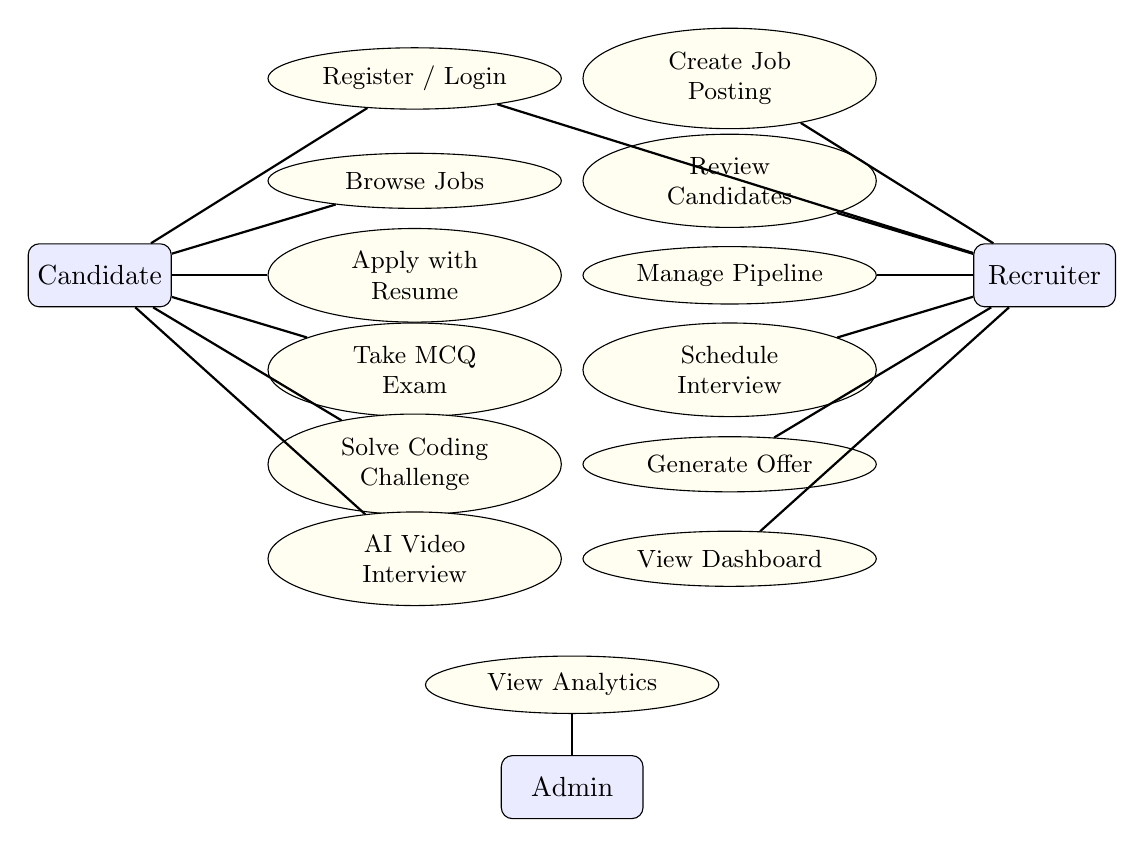
\begin{tikzpicture}[
  actor/.style={rectangle, draw, rounded corners, minimum width=1.8cm, minimum height=0.8cm, fill=blue!8},
  usecase/.style={ellipse, draw, minimum width=2.8cm, minimum height=0.7cm, text width=2.4cm, align=center, font=\small, fill=yellow!6},
  line/.style={draw, thick}
]
  \node[actor] (cand) at (0,0) {Candidate};
  \node[actor] (rec)  at (12,0) {Recruiter};
  \node[actor] (admin) at (6,-6.5) {Admin};

  \node[usecase] (uc1) at (4, 2.5)  {Register / Login};
  \node[usecase] (uc2) at (4, 1.2)  {Browse Jobs};
  \node[usecase] (uc3) at (4, 0)    {Apply with Resume};
  \node[usecase] (uc4) at (4,-1.2)  {Take MCQ Exam};
  \node[usecase] (uc5) at (4,-2.4)  {Solve Coding Challenge};
  \node[usecase] (uc6) at (4,-3.6)  {AI Video Interview};

  \node[usecase] (uc7) at (8, 2.5)  {Create Job Posting};
  \node[usecase] (uc8) at (8, 1.2)  {Review Candidates};
  \node[usecase] (uc9) at (8, 0)    {Manage Pipeline};
  \node[usecase] (uc10) at (8,-1.2) {Schedule Interview};
  \node[usecase] (uc11) at (8,-2.4) {Generate Offer};
  \node[usecase] (uc12) at (8,-3.6) {View Dashboard};

  \node[usecase] (uc13) at (6,-5.2) {View Analytics};

  \path[line] (cand) -- (uc1);
  \path[line] (cand) -- (uc2);
  \path[line] (cand) -- (uc3);
  \path[line] (cand) -- (uc4);
  \path[line] (cand) -- (uc5);
  \path[line] (cand) -- (uc6);

  \path[line] (rec) -- (uc1);
  \path[line] (rec) -- (uc7);
  \path[line] (rec) -- (uc8);
  \path[line] (rec) -- (uc9);
  \path[line] (rec) -- (uc10);
  \path[line] (rec) -- (uc11);
  \path[line] (rec) -- (uc12);

  \path[line] (admin) -- (uc13);
\end{tikzpicture}
}
\caption{Use case diagram showing primary actor interactions}
\label{fig:usecase}
\end{figure}

\section{Technology Stack}
\label{sec:techstack}

SmartHire is architected using a modern full-stack web technology stack designed for high developer productivity, type safety, low latency, and seamless scalability. The application leverages Next.js~15's App Router architecture on the frontend, combined with React~19 and TypeScript~5 for building type-safe, component-driven user interfaces. Styling is implemented using Tailwind CSS for rapid, uniform UI design, supported by Lucide React for consistent icon design.

The core database and authentication infrastructure is powered by Supabase PostgreSQL, offering managed relational storage, Row-Level Security (RLS) policies, and integrated JWT authentication. Interactive technical evaluations rely on the Monaco Editor engine for browser-based code editing, while AI evaluations are executed using Google's Gemini API for resume ATS parsing and interview scorecard generation. Table~\ref{tab:techstack} summarizes the complete technology stack across all architectural layers.

\begin{table}[htbp]
\centering
\caption{Technology stack}
\label{tab:techstack}
\small
\begin{tabular}{p{1.6in}p{1.2in}p{2.8in}}
\toprule
\textbf{Layer}       & \textbf{Technology}    & \textbf{Rationale} \\
\midrule
Frontend Framework   & Next.js 15             & Server-side rendering, file-based routing, API routes \\
UI Library           & React 19               & Component-based architecture, concurrent rendering \\
Language             & TypeScript 5           & Static type checking reduces runtime errors \\
Styling              & Tailwind CSS           & Utility-first CSS framework for rapid UI development \\
Icons                & Lucide React           & Consistent, lightweight SVG icon set \\
Code Editor          & Monaco Editor          & VS Code engine; syntax highlighting, IntelliSense \\
Backend/Database     & Supabase PostgreSQL    & Managed PostgreSQL with auth, RLS, real-time \\
AI Engine            & Google Gemini API      & Multimodal LLM for resume scoring and interview evaluation \\
PDF Generation       & jsPDF + html2canvas    & Client-side vector PDF rendering \\
Deployment           & Vercel                 & Serverless edge deployment with global CDN \\
Version Control      & Git + GitHub           & Collaborative source code management \\
Package Manager      & pnpm                   & Fast, disk-efficient dependency management \\
\bottomrule
\end{tabular}
\end{table}

\section{Hardware and Software Requirements}
\label{sec:hw-sw}

\subsection{Development Environment}

Setting up the local development environment requires a modern 64-bit workstation operating system capable of running Node.js~18+ and managing monorepo workspace dependencies. Developer machines require at least 8~GB of RAM (16~GB recommended) to comfortably run concurrent development servers, browser developer tools, and Visual Studio Code extensions.

Local development relies on pnpm workspaces for fast, disk-efficient package management across the repository. Developers configure local environment variables (\texttt{.env.local}) to connect to Supabase development instances and Google Gemini API endpoints. Table~\ref{tab:dev-env} outlines the hardware and software specifications for the development environment.

\begin{table}[htbp]
\centering
\caption{Development environment requirements}
\label{tab:dev-env}
\small
\begin{tabular}{p{2in}p{3.5in}}
\toprule
\textbf{Requirement} & \textbf{Specification} \\
\midrule
Operating System     & Windows 10/11 or Ubuntu 22.04 LTS \\
Processor            & Intel Core i5 or equivalent (minimum) \\
RAM                  & 8 GB minimum; 16 GB recommended \\
Storage              & 20 GB free disk space \\
Node.js              & v18.x or later \\
Browser              & Chrome 120+ or Firefox 120+ \\
IDE                  & Visual Studio Code 1.85+ \\
\bottomrule
\end{tabular}
\end{table}

\subsection{Production Environment}

The production deployment runs on Vercel's serverless infrastructure, which provisions compute resources on demand. The database is hosted on Supabase's managed PostgreSQL service. No dedicated server hardware is required.

\section{Constraints and Assumptions}
\label{sec:constraints}

\begin{itemize}[leftmargin=1.5em]
  \item The system assumes that all candidate resumes are uploaded as PDF files. Other document formats (DOCX, ODT) are not supported in the current version.
  \item AI-based evaluation via Gemini API requires an active internet connection and a valid API key. API rate limits may constrain throughput during peak usage.
  \item The coding assessment module currently supports JavaScript and Python. Additional languages require backend execution environment configuration.
  \item The platform is designed for English-language content. Localisation is outside the scope of the current version.
\end{itemize}

\section{Risk Analysis}
\label{sec:risk}

Developing an autonomous recruitment platform involves navigating technical, operational, and security risks. Technical risks center on external API reliance (such as rate limits or transient outages on the Google Gemini API), database connection pool exhaustion under high application submission loads, and variations in candidate resume formatting that challenge PDF text extraction heuristics. Operational and security risks include potential cross-tenant data exposure and browser compatibility issues across candidate devices.

To mitigate these risks, SmartHire incorporates defensive architectural patterns: API request queues with exponential backoff retries, connection pooling via PgBouncer on Supabase, candidate resume text preview/editing capabilities prior to submission, strict PostgreSQL Row-Level Security (RLS) policies, and comprehensive automated test suites. Table~\ref{tab:risk} presents the risk assessment matrix detailing identified risks, their likelihood and impact levels, and implemented mitigation strategies.

\begin{table}[htbp]
\centering
\caption{Risk assessment matrix}
\label{tab:risk}
\small
\begin{tabular}{p{2in}ccp{2.2in}}
\toprule
\textbf{Risk} & \textbf{Likelihood} & \textbf{Impact} & \textbf{Mitigation} \\
\midrule
API rate limiting (Gemini) & Medium & Medium & Queue requests; implement exponential backoff \\
Database connection pooling exhaustion & Low & High & Use Supabase connection pooler; limit concurrent queries \\
Resume parsing inaccuracy & Medium & Medium & Validate parsed output; allow candidate correction \\
Cross-tenant data leakage & Low & Critical & RLS policies; schema-level isolation; integration tests \\
Browser compatibility issues & Low & Low & Target latest two versions of Chrome and Firefox \\
\bottomrule
\end{tabular}
\end{table}


\makechaptertitlepage{4}{SYSTEM DESIGN AND ARCHITECTURE}
\setcounter{chapter}{3}
\chapter{System Design and Architecture}
\label{ch:design}

\section{Architectural Overview}
\label{sec:arch-overview}

SmartHire follows a layered architecture comprising four tiers: a client-side presentation layer, an application logic layer, an AI services layer, and a data persistence layer. This separation allows each tier to evolve independently and simplifies testing. The presentation layer is a Next.js~15 single-page application that communicates with the backend through RESTful API routes. The application logic layer, also implemented within Next.js using its App Router API routes, handles request validation, business logic, and database interaction. The AI services layer wraps calls to Google's Gemini API for resume scoring and interview evaluation. The data persistence layer is a managed PostgreSQL instance on Supabase, organised into domain-specific schemas.

\begin{figure}[htbp]
\centering
\resizebox{0.95\textwidth}{!}{
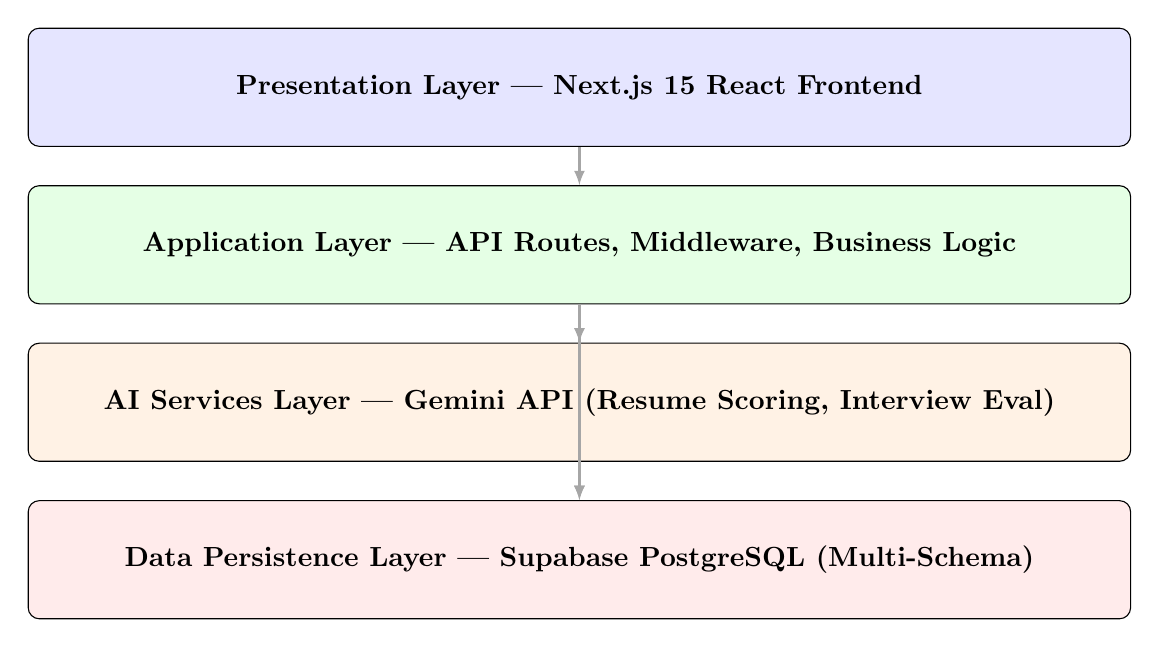
\begin{tikzpicture}[
  tier/.style={rectangle, draw, rounded corners, fill=#1, minimum width=14cm, minimum height=1.5cm, text centered, font=\bfseries},
  arrow/.style={-latex, thick, draw=gray!70}
]
  \node[tier=blue!10]   (pres) at (0,6)  {Presentation Layer --- Next.js 15 React Frontend};
  \node[tier=green!10]  (app)  at (0,4)  {Application Layer --- API Routes, Middleware, Business Logic};
  \node[tier=orange!10] (ai)   at (0,2)  {AI Services Layer --- Gemini API (Resume Scoring, Interview Eval)};
  \node[tier=red!8]     (data) at (0,0)  {Data Persistence Layer --- Supabase PostgreSQL (Multi-Schema)};

  \draw[arrow] (pres) -- (app);
  \draw[arrow] (app) -- (ai);
  \draw[arrow] (app) -- (data);
  \draw[arrow] (ai) -- (data);
\end{tikzpicture}
}
\caption{Four-tier layered architecture of SmartHire}
\label{fig:layered-arch}
\end{figure}

Figure~\ref{fig:layered-arch} illustrates the four tiers and their communication paths. The presentation layer issues HTTP requests to the application layer. The application layer may, depending on the endpoint, invoke the AI services layer (for operations requiring Gemini evaluation) or interact directly with the database. The AI services layer also reads from and writes to the database---for example, storing computed ATS scores alongside the corresponding application record.

\section{High-Level System Architecture}
\label{sec:highlevel}

\begin{figure}[htbp]
\centering
\resizebox{0.95\textwidth}{!}{
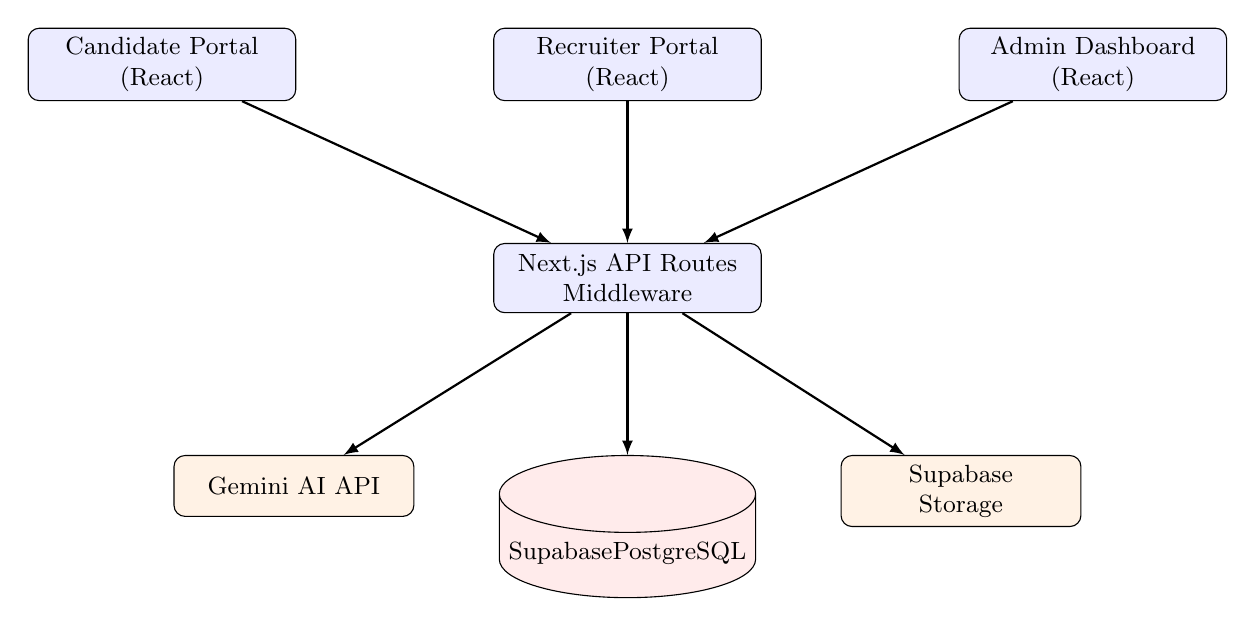
\begin{tikzpicture}[node distance=1.4cm, auto,
  comp/.style={rectangle, draw, rounded corners, fill=blue!8, text width=9em, text centered, minimum height=2.5em, font=\small},
  db/.style={cylinder, draw, shape border rotate=90, fill=red!8, minimum height=2em, minimum width=3em, aspect=0.3, font=\small},
  ext/.style={rectangle, draw, rounded corners, fill=orange!10, text width=8em, text centered, minimum height=2.2em, font=\small},
  arrow/.style={-latex, thick}
]
  \node[comp] (candidateUI) {Candidate Portal\\(React)};
  \node[comp, right=2.5cm of candidateUI] (recruiterUI) {Recruiter Portal\\(React)};
  \node[comp, right=2.5cm of recruiterUI] (adminUI) {Admin Dashboard\\(React)};

  \node[comp, below=1.8cm of recruiterUI] (apiLayer) {Next.js API Routes\\Middleware};

  \node[ext, below left=1.8cm and 1cm of apiLayer]  (gemini) {Gemini AI API};
  \node[db,  below=1.8cm of apiLayer]                (db)     {Supabase\\PostgreSQL};
  \node[ext, below right=1.8cm and 1cm of apiLayer] (storage) {Supabase\\Storage};

  \draw[arrow] (candidateUI) -- (apiLayer);
  \draw[arrow] (recruiterUI) -- (apiLayer);
  \draw[arrow] (adminUI)     -- (apiLayer);
  \draw[arrow] (apiLayer)    -- (gemini);
  \draw[arrow] (apiLayer)    -- (db);
  \draw[arrow] (apiLayer)    -- (storage);
\end{tikzpicture}
}
\caption{High-level component architecture}
\label{fig:highlevel}
\end{figure}

The high-level architecture (Figure~\ref{fig:highlevel}) shows the three frontend portals connecting to a shared API layer. The API layer mediates all access to external services (Gemini API) and storage backends (PostgreSQL database and Supabase file storage). This design ensures that frontend components never interact with the database directly, centralising access control and validation logic in the API layer.

\section{Database Design}
\label{sec:db-design}

\subsection{Multi-Schema Organisation}

SmartHire's PostgreSQL database is divided into domain-specific schemas rather than placing all tables in a single \texttt{public} schema. This design decision offers three advantages: logical grouping of related entities, simplified access control policies, and reduced risk of naming collisions as the system grows.

\begin{figure}[htbp]
\centering
\resizebox{0.95\textwidth}{!}{
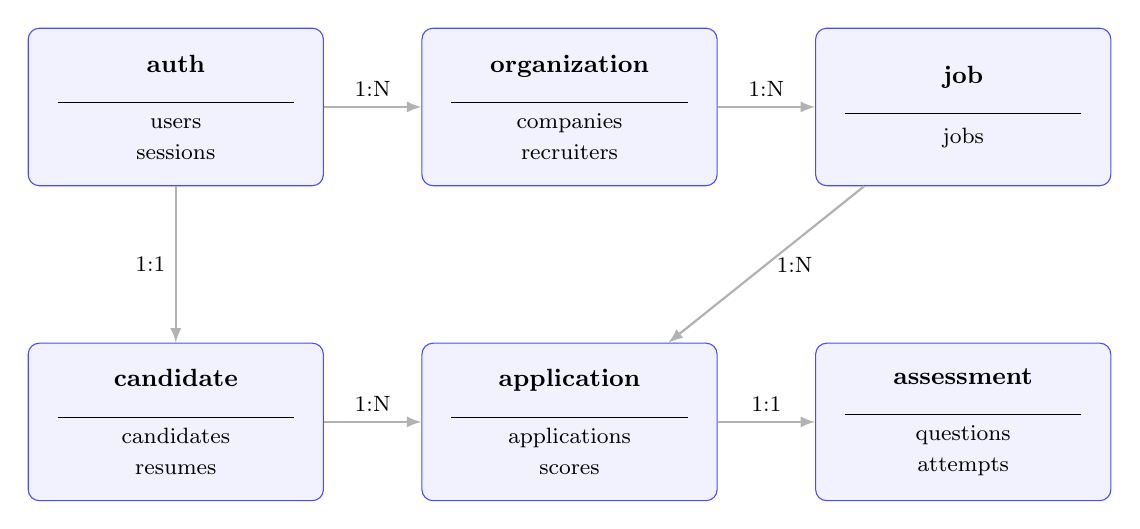
\begin{tikzpicture}[
  schema/.style={rectangle, draw=blue!70, fill=blue!5, rounded corners, text width=10em, text centered, minimum height=2cm, font=\small},
  arrow/.style={-latex, thick, draw=gray!60}
]
  \node[schema] (auth) at (0,4) {\textbf{auth}\\\rule{3cm}{0.3pt}\\\footnotesize users\\\footnotesize sessions};
  \node[schema] (org)  at (5,4) {\textbf{organization}\\\rule{3cm}{0.3pt}\\\footnotesize companies\\\footnotesize recruiters};
  \node[schema] (job)  at (10,4) {\textbf{job}\\\rule{3cm}{0.3pt}\\\footnotesize jobs};
  \node[schema] (cand) at (0,0) {\textbf{candidate}\\\rule{3cm}{0.3pt}\\\footnotesize candidates\\\footnotesize resumes};
  \node[schema] (app)  at (5,0) {\textbf{application}\\\rule{3cm}{0.3pt}\\\footnotesize applications\\\footnotesize scores};
  \node[schema] (assess) at (10,0) {\textbf{assessment}\\\rule{3cm}{0.3pt}\\\footnotesize questions\\\footnotesize attempts};

  \draw[arrow] (auth) -- (org) node[midway, above, font=\footnotesize] {1:N};
  \draw[arrow] (org)  -- (job) node[midway, above, font=\footnotesize] {1:N};
  \draw[arrow] (auth) -- (cand) node[midway, left, font=\footnotesize] {1:1};
  \draw[arrow] (job)  -- (app) node[midway, right, font=\footnotesize] {1:N};
  \draw[arrow] (cand) -- (app) node[midway, above, font=\footnotesize] {1:N};
  \draw[arrow] (app) -- (assess) node[midway, above, font=\footnotesize] {1:1};
\end{tikzpicture}
}
\caption{Multi-schema database organisation with entity relationships}
\label{fig:schema}
\end{figure}

\subsection{Entity Descriptions}

Table~\ref{tab:entities} summarises the principal database entities and their key attributes.

\begin{table}[htbp]
\centering
\caption{Principal database entities}
\label{tab:entities}
\small
\begin{tabular}{p{1.2in}p{1in}p{3.3in}}
\toprule
\textbf{Schema} & \textbf{Table} & \textbf{Key Attributes} \\
\midrule
\texttt{auth}        & \texttt{users}        & id, email, encrypted\_password, role, created\_at \\
\texttt{organization}& \texttt{companies}    & id, name, industry, website, logo\_url \\
\texttt{organization}& \texttt{recruiters}   & id, user\_id (FK), company\_id (FK), position \\
\texttt{job}         & \texttt{jobs}         & id, recruiter\_id (FK), title, description, skills[], status, location, salary\_range \\
\texttt{candidate}   & \texttt{candidates}   & id, user\_id (FK), phone, skills[], experience\_years \\
\texttt{candidate}   & \texttt{resumes}      & id, candidate\_id (FK), file\_url, parsed\_text, parsed\_at \\
\texttt{application} & \texttt{applications} & id, job\_id (FK), candidate\_id (FK), stage, ats\_score, mcq\_score, coding\_score, interview\_score, status \\
\texttt{assessment}  & \texttt{questions}    & id, job\_id (FK), type (mcq/coding), content, options[], correct\_answer, difficulty \\
\texttt{assessment}  & \texttt{attempts}     & id, application\_id (FK), question\_id (FK), answer, is\_correct, score, submitted\_at \\
\bottomrule
\end{tabular}
\end{table}

\subsection{Entity-Relationship Diagram}

Figure~\ref{fig:er} presents the complete ER diagram for the database, showing primary keys, foreign keys, and cardinality.

\begin{figure}[htbp]
\centering
\resizebox{0.95\textwidth}{!}{
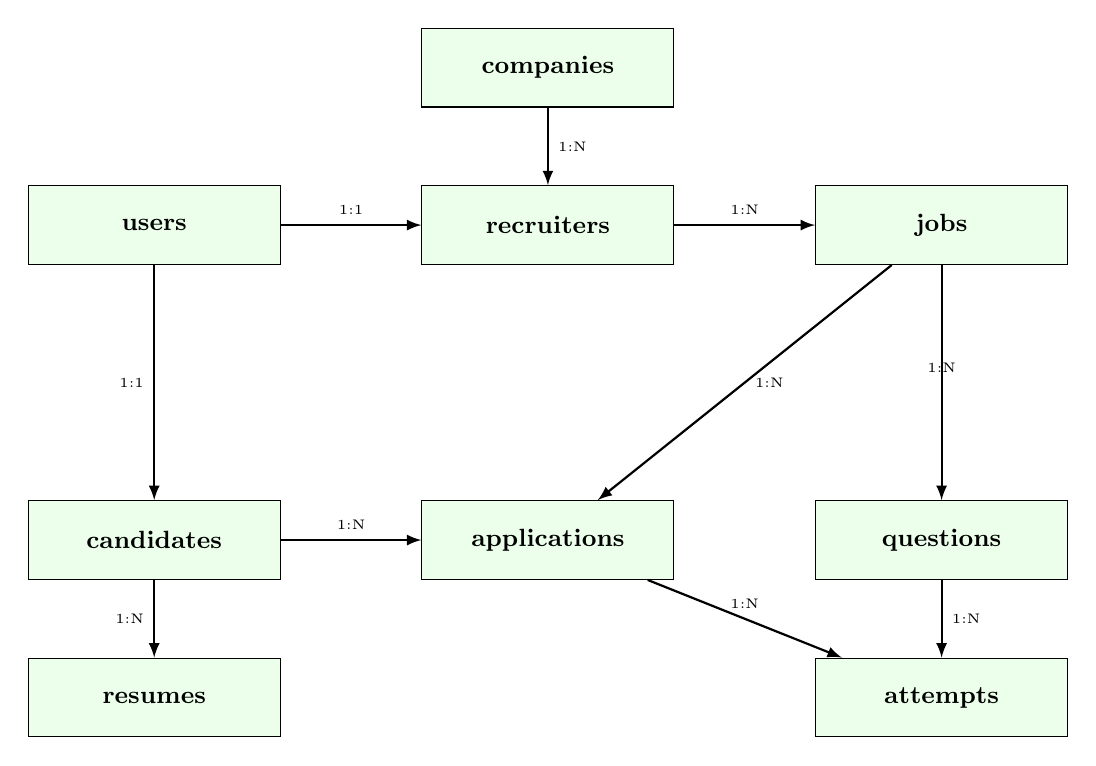
\begin{tikzpicture}[
  entity/.style={rectangle, draw, fill=green!8, minimum width=3.2cm, minimum height=1cm, font=\small\bfseries},
  rel/.style={diamond, draw, fill=yellow!15, minimum width=1.5cm, aspect=2, font=\footnotesize},
  arrow/.style={-latex, thick}
]
  \node[entity] (user) at (0,6) {users};
  \node[entity] (company) at (5,8) {companies};
  \node[entity] (recruiter) at (5,6) {recruiters};
  \node[entity] (job) at (10,6) {jobs};
  \node[entity] (candidate) at (0,2) {candidates};
  \node[entity] (resume) at (0,0) {resumes};
  \node[entity] (application) at (5,2) {applications};
  \node[entity] (question) at (10,2) {questions};
  \node[entity] (attempt) at (10,0) {attempts};

  \draw[arrow] (user) -- (recruiter) node[midway,above,font=\tiny]{1:1};
  \draw[arrow] (company) -- (recruiter) node[midway,right,font=\tiny]{1:N};
  \draw[arrow] (recruiter) -- (job) node[midway,above,font=\tiny]{1:N};
  \draw[arrow] (user) -- (candidate) node[midway,left,font=\tiny]{1:1};
  \draw[arrow] (candidate) -- (resume) node[midway,left,font=\tiny]{1:N};
  \draw[arrow] (candidate) -- (application) node[midway,above,font=\tiny]{1:N};
  \draw[arrow] (job) -- (application) node[midway,right,font=\tiny]{1:N};
  \draw[arrow] (job) -- (question) node[midway,above,font=\tiny]{1:N};
  \draw[arrow] (application) -- (attempt) node[midway,above,font=\tiny]{1:N};
  \draw[arrow] (question) -- (attempt) node[midway,right,font=\tiny]{1:N};
\end{tikzpicture}
}
\caption{Entity-Relationship diagram}
\label{fig:er}
\end{figure}

\section{Data Flow Diagrams}
\label{sec:dfd}

\subsection{DFD Level 0 --- Context Diagram}

The context diagram (Figure~\ref{fig:dfd0}) represents SmartHire as a single process interacting with three external entities: Candidate, Recruiter, and the Gemini AI service.

\begin{figure}[htbp]
\centering
\resizebox{0.95\textwidth}{!}{
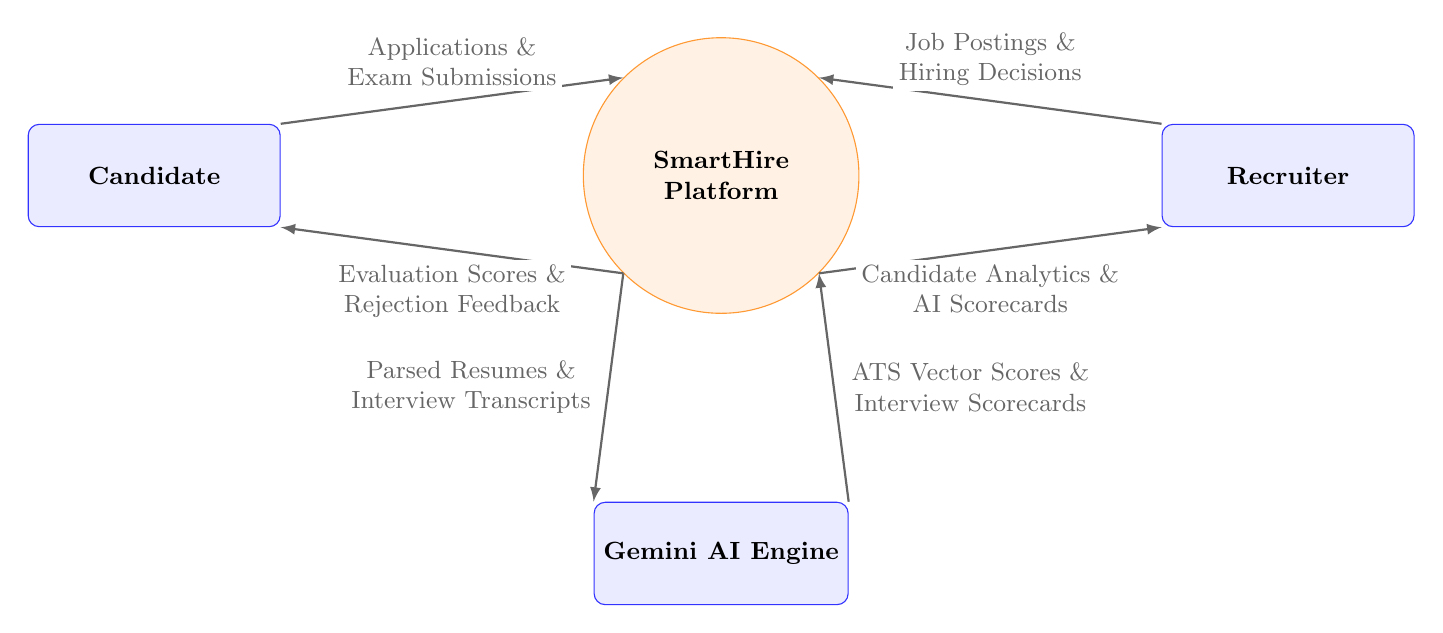
\begin{tikzpicture}[
  ext/.style={rectangle, draw=blue!80, fill=blue!8, minimum width=3.2cm, minimum height=1.3cm, rounded corners, font=\small\bfseries, align=center},
  process/.style={circle, draw=orange!80, fill=orange!10, minimum size=3.5cm, font=\small\bfseries, text width=2.8cm, align=center},
  arrow/.style={-latex, thick, color=gray!80!black},
  lbl/.style={font=\small, align=center, fill=white, inner sep=2pt}
]
  \node[ext] (cand) at (-7.2, 0) {Candidate};
  \node[process] (sys) at (0, 0) {SmartHire\\Platform};
  \node[ext] (rec) at (7.2, 0) {Recruiter};
  \node[ext] (ai) at (0, -4.8) {Gemini AI Engine};

  % Candidate <-> System
  \draw[arrow] (cand.north east) -- (sys.north west) node[midway, above=3pt, lbl] {Applications \&\\Exam Submissions};
  \draw[arrow] (sys.south west) -- (cand.south east) node[midway, below=3pt, lbl] {Evaluation Scores \&\\Rejection Feedback};

  % Recruiter <-> System
  \draw[arrow] (rec.north west) -- (sys.north east) node[midway, above=3pt, lbl] {Job Postings \&\\Hiring Decisions};
  \draw[arrow] (sys.south east) -- (rec.south west) node[midway, below=3pt, lbl] {Candidate Analytics \&\\AI Scorecards};

  % System <-> Gemini AI
  \draw[arrow] (sys.south west) -- (ai.north west) node[midway, left=4pt, lbl] {Parsed Resumes \&\\Interview Transcripts};
  \draw[arrow] (ai.north east) -- (sys.south east) node[midway, right=4pt, lbl] {ATS Vector Scores \&\\Interview Scorecards};
\end{tikzpicture}
}
\caption{DFD Level 0 --- Context diagram}
\label{fig:dfd0}
\end{figure}

\subsection{DFD Level 1}

Figure~\ref{fig:dfd1} decomposes the system into its six principal processing modules, showing data flows between them and the data stores.

\begin{figure}[htbp]
\centering
\resizebox{0.95\textwidth}{!}{
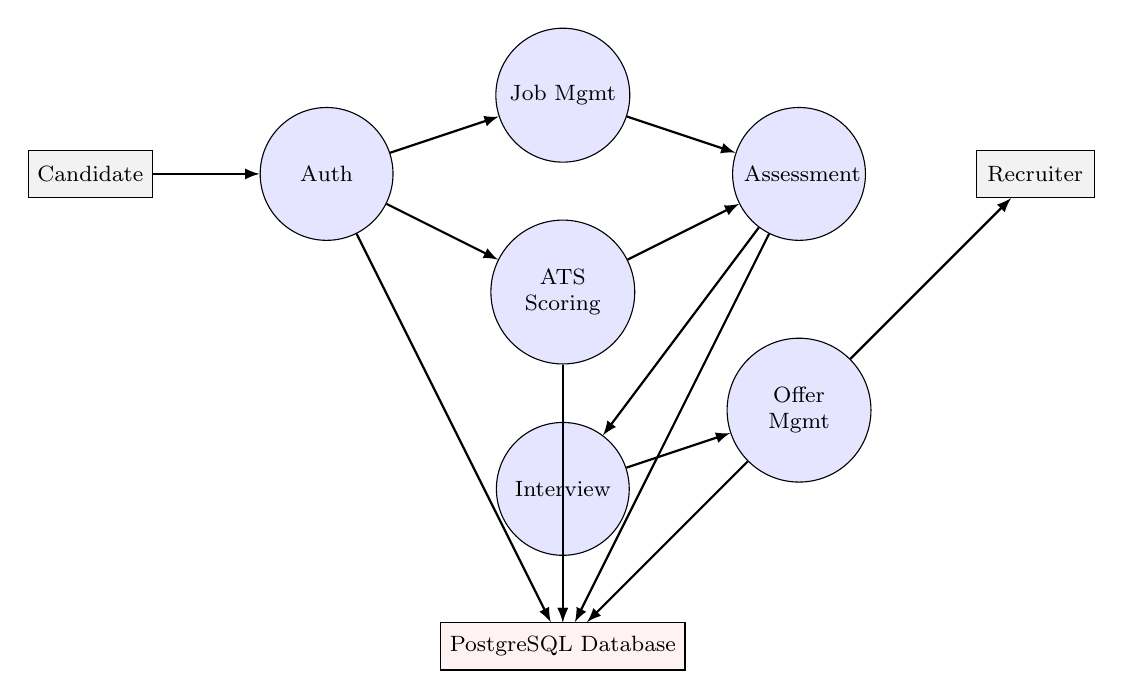
\begin{tikzpicture}[
  process/.style={circle, draw, fill=blue!10, minimum size=1.4cm, font=\footnotesize, text width=1.4cm, align=center},
  store/.style={rectangle, draw, fill=red!5, minimum width=2cm, minimum height=0.6cm, font=\footnotesize},
  ext/.style={rectangle, draw, fill=gray!10, minimum width=1.5cm, minimum height=0.6cm, font=\footnotesize},
  arrow/.style={-latex, thick, font=\tiny}
]
  \node[ext] (cand) at (-4,3) {Candidate};
  \node[ext] (rec)  at (8,3) {Recruiter};

  \node[process] (p1) at (-1,3) {Auth};
  \node[process] (p2) at (2,4) {Job Mgmt};
  \node[process] (p3) at (2,1.5) {ATS Scoring};
  \node[process] (p4) at (5,3) {Assessment};
  \node[process] (p5) at (2,-1) {Interview};
  \node[process] (p6) at (5,0) {Offer Mgmt};

  \node[store] (db) at (2,-3) {PostgreSQL Database};

  \draw[arrow] (cand) -- (p1);
  \draw[arrow] (p1) -- (p2);
  \draw[arrow] (p1) -- (p3);
  \draw[arrow] (p2) -- (p4);
  \draw[arrow] (p3) -- (p4);
  \draw[arrow] (p4) -- (p5);
  \draw[arrow] (p5) -- (p6);
  \draw[arrow] (p6) -- (rec);
  \draw[arrow] (p1) -- (db);
  \draw[arrow] (p3) -- (db);
  \draw[arrow] (p4) -- (db);
  \draw[arrow] (p5) -- (db);
  \draw[arrow] (p6) -- (db);
\end{tikzpicture}
}
\caption{DFD Level 1 --- Module decomposition}
\label{fig:dfd1}
\end{figure}

\section{Sequence Diagrams}
\label{sec:sequence}

\subsection{Candidate Application Flow}

The following sequence describes the interactions when a candidate applies for a job:

\begin{enumerate}[leftmargin=1.5em]
  \item Candidate uploads a PDF resume via the application form.
  \item The frontend sends a POST request to \texttt{/api/applications} with the resume file.
  \item The API route stores the resume in Supabase Storage and triggers the resume parsing service.
  \item The parsing service extracts text from the PDF, identifies skills and experience, and stores the parsed data.
  \item The ATS scoring module computes a relevance score by comparing parsed skills against the job's required skills.
  \item The computed score and parsed data are persisted in the \texttt{application.applications} table.
  \item A confirmation response is sent back to the candidate portal.
\end{enumerate}

\subsection{Recruiter Pipeline Management}

When a recruiter moves a candidate from one pipeline stage to another:

\begin{enumerate}[leftmargin=1.5em]
  \item The recruiter drags a candidate card on the Kanban board from the current stage column to the target stage column.
  \item The frontend issues a PATCH request to \texttt{/api/applications/\{id\}} with the new stage value.
  \item The API route validates that the transition is legal (stages can only advance forward, not backward) and updates the database.
  \item If the candidate is moved to a rejection stage, a rejection reason is recorded.
  \item The updated application state is returned to the frontend, and the Kanban board re-renders.
\end{enumerate}

\section{Authentication Workflow}
\label{sec:auth-workflow}

SmartHire delegates authentication to Supabase Auth, which provides JWT-based session management. Figure~\ref{fig:auth-flow} outlines the registration and login sequence.

\begin{figure}[htbp]
\centering
\resizebox{0.95\textwidth}{!}{
\begin{tikzpicture}[
  step/.style={rectangle, draw=blue!70, fill=blue!5, rounded corners, text width=9.0em, text centered, minimum height=2.8em, font=\small},
  decision/.style={diamond, draw=orange!80, fill=orange!10, text width=7.0em, text centered, aspect=2.2, font=\small},
  arrow/.style={-latex, thick, color=gray!80!black},
  lbl/.style={font=\small\bfseries, fill=white, inner sep=2pt}
]
  \node[step] (start) at (0,0) {User Login Request};
  \node[step] (submit) at (4.5,0) {Submit Credentials};
  \node[decision] (check) at (9.5,0) {Credentials Valid?};
  \node[step] (jwt) at (14.8,0) {Issue JWT Token};
  \node[step] (redirect) at (14.8,-2.8) {Redirect to Portal};
  \node[step] (error) at (9.5,-2.8) {Return Auth Error};

  \draw[arrow] (start) -- (submit);
  \draw[arrow] (submit) -- (check);
  \draw[arrow] (check) -- node[above=2pt, lbl]{Yes} (jwt);
  \draw[arrow] (check) -- node[right=4pt, lbl]{No} (error);
  \draw[arrow] (jwt) -- (redirect);
\end{tikzpicture}
}
\caption{Authentication workflow}
\label{fig:auth-flow}
\end{figure}

\section{ATS Resume Scoring Workflow}
\label{sec:ats-workflow}

The ATS scoring process operates in two phases: text extraction and relevance computation.

\textbf{Phase 1: Text Extraction.} When a candidate uploads a PDF resume, the system uses a text extraction library to convert the document into plain text. The extracted text is stored in the \texttt{candidate.resumes} table alongside the original file URL.

\textbf{Phase 2: Relevance Scoring.} The extracted resume text and the job description are sent to the Gemini API with a structured prompt requesting a relevance assessment. The API returns a composite score (0--10) along with dimensional breakdowns for skills match, experience relevance, and qualification alignment. These scores are recorded in the \texttt{application.applications} table.

\section{Coding Assessment Workflow}
\label{sec:coding-workflow}

\begin{figure}[htbp]
\centering
\resizebox{0.95\textwidth}{!}{
\begin{tikzpicture}[
  step/.style={rectangle, draw=teal!80, fill=teal!5, rounded corners, text width=9.5em, text centered, minimum height=2.5em, font=\small},
  arrow/.style={-latex, thick, color=gray!80!black}
]
  \node[step] (open) at (0,0) {Open Monaco IDE};
  \node[step] (editor) at (4.2,0) {Write Code Solution};
  \node[step] (submit) at (8.4,0) {Click Submit Solution};
  \node[step] (exec) at (8.4,-2.2) {Execute Against Test Cases};
  \node[step] (result) at (4.2,-2.2) {Evaluate Output Results};
  \node[step] (score) at (0,-2.2) {Record Score in DB};

  \draw[arrow] (open) -- (editor);
  \draw[arrow] (editor) -- (submit);
  \draw[arrow] (submit) -- (exec);
  \draw[arrow] (exec) -- (result);
  \draw[arrow] (result) -- (score);
\end{tikzpicture}
}
\caption{Coding assessment execution workflow}
\label{fig:coding-flow}
\end{figure}

The coding assessment module (Figure~\ref{fig:coding-flow}) presents candidates with a problem description alongside a Monaco editor instance. Candidates write their solution and click ``Run'' to execute against visible sample test cases, or ``Submit'' to evaluate against the complete hidden test suite. The server runs the code, captures stdout, compares it against expected outputs, and computes a score based on the proportion of test cases passed.

\section{AI Video Interview Workflow}
\label{sec:interview-workflow}

The AI interview module presents a sequence of pre-configured questions to the candidate. For each question, the candidate records a video response through the browser's media capture API. Once all responses are recorded, the audio is transcribed and the transcriptions are sent to the Gemini API along with the original questions. The API evaluates each response across dimensions such as technical accuracy, communication clarity, and depth of reasoning, and returns a structured scorecard with per-dimension ratings and an overall recommendation (\texttt{strong\_hire}, \texttt{hire}, \texttt{neutral}, \texttt{no\_hire}, \texttt{strong\_no\_hire}).

\section{Deployment Architecture}
\label{sec:deployment}

SmartHire is deployed using a serverless architecture:

\begin{itemize}[leftmargin=1.5em]
  \item \textbf{Frontend and API}: Deployed on Vercel, which provisions serverless functions for each API route and serves static assets through a global CDN.
  \item \textbf{Database}: Hosted on Supabase's managed PostgreSQL service with connection pooling via PgBouncer.
  \item \textbf{File Storage}: Resume PDFs and generated offer letters are stored in Supabase Storage buckets with signed URL access.
  \item \textbf{AI Services}: Google Gemini API is accessed via HTTPS. API keys are stored as environment variables and never exposed to the client.
\end{itemize}

This architecture eliminates the need for server provisioning, scaling configuration, or uptime monitoring. Vercel scales automatically based on incoming traffic, and Supabase handles database maintenance, backups, and connection management.

\section{DFD Level 2 --- ATS Scoring Subsystem}
\label{sec:dfd2}

Figure~\ref{fig:dfd2} expands the ATS scoring process from DFD Level~1 into its constituent sub-processes. This decomposition reveals the internal pipeline through which a candidate's resume is transformed from an uploaded PDF file into a normalised relevance score stored alongside the application record.

\begin{figure}[htbp]
\centering
\resizebox{0.95\textwidth}{!}{
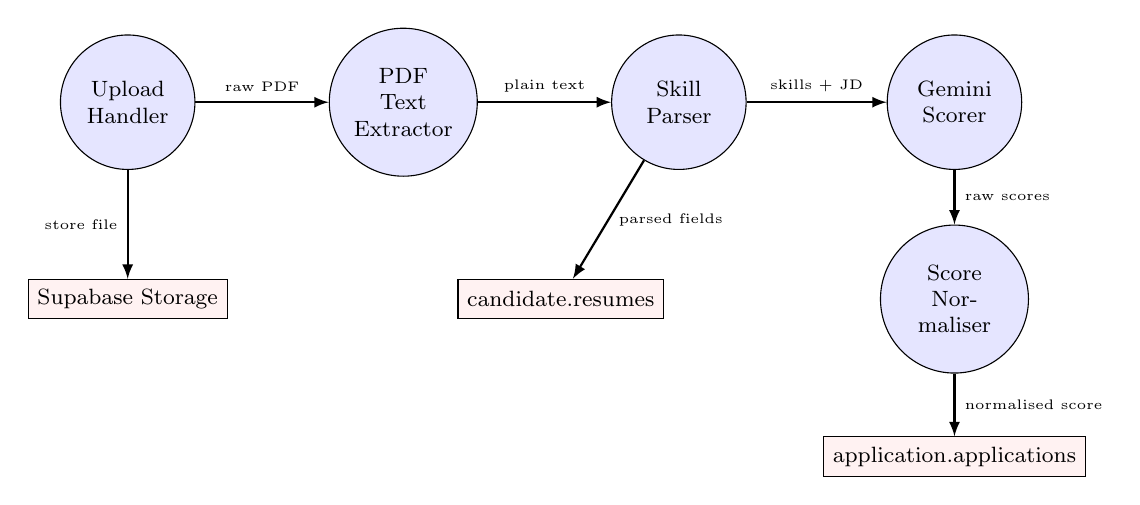
\begin{tikzpicture}[
  process/.style={circle, draw, fill=blue!10, minimum size=1.2cm, font=\footnotesize, text width=1.3cm, align=center},
  store/.style={rectangle, draw, fill=red!5, minimum width=1.8cm, minimum height=0.5cm, font=\footnotesize},
  arrow/.style={-latex, thick, font=\tiny}
]
  \node[process] (p1) at (0,2)   {Upload Handler};
  \node[process] (p2) at (3.5,2) {PDF Text Extractor};
  \node[process] (p3) at (7,2)   {Skill Parser};
  \node[process] (p4) at (10.5,2) {Gemini Scorer};
  \node[process] (p5) at (10.5,-0.5) {Score Normaliser};

  \node[store] (s1) at (0,-0.5) {Supabase Storage};
  \node[store] (s2) at (5.5,-0.5) {candidate.resumes};
  \node[store] (s3) at (10.5,-2.5) {application.applications};

  \draw[arrow] (p1) -- (p2) node[midway, above] {raw PDF};
  \draw[arrow] (p1) -- (s1) node[midway, left] {store file};
  \draw[arrow] (p2) -- (p3) node[midway, above] {plain text};
  \draw[arrow] (p3) -- (s2) node[midway, right] {parsed fields};
  \draw[arrow] (p3) -- (p4) node[midway, above] {skills + JD};
  \draw[arrow] (p4) -- (p5) node[midway, right] {raw scores};
  \draw[arrow] (p5) -- (s3) node[midway, right] {normalised score};
\end{tikzpicture}
}
\caption{DFD Level 2 --- ATS scoring subsystem decomposition}
\label{fig:dfd2}
\end{figure}

The upload handler receives the PDF file from the candidate's browser, validates the file type and size, and stores the original document in Supabase Storage. The PDF text extractor converts the binary PDF into plain text, handling common formatting challenges such as multi-column layouts and header/footer artifacts. The skill parser identifies technical skills, educational qualifications, and experience durations from the extracted text using pattern matching and NLP heuristics. The parsed fields are stored in the \texttt{candidate.resumes} table for future reference.

The Gemini scorer then receives the parsed skills and the job description, constructs a structured evaluation prompt, and sends it to the Gemini API. The API returns dimensional scores (skills match, experience relevance, overall fit) as floating-point values. The score normaliser validates the returned values, clamps them to the 0--10 range, and persists the final composite score in the \texttt{application.applications} table.

\section{Activity Diagram --- Candidate Application Lifecycle}
\label{sec:activity}

Figure~\ref{fig:activity} models the complete lifecycle of a candidate's interaction with SmartHire, from initial registration through to offer acceptance or rejection. Decision points represent system-enforced thresholds that determine whether a candidate advances to the next evaluation stage.

\begin{figure}[htbp]
\centering
\resizebox{0.95\textwidth}{!}{
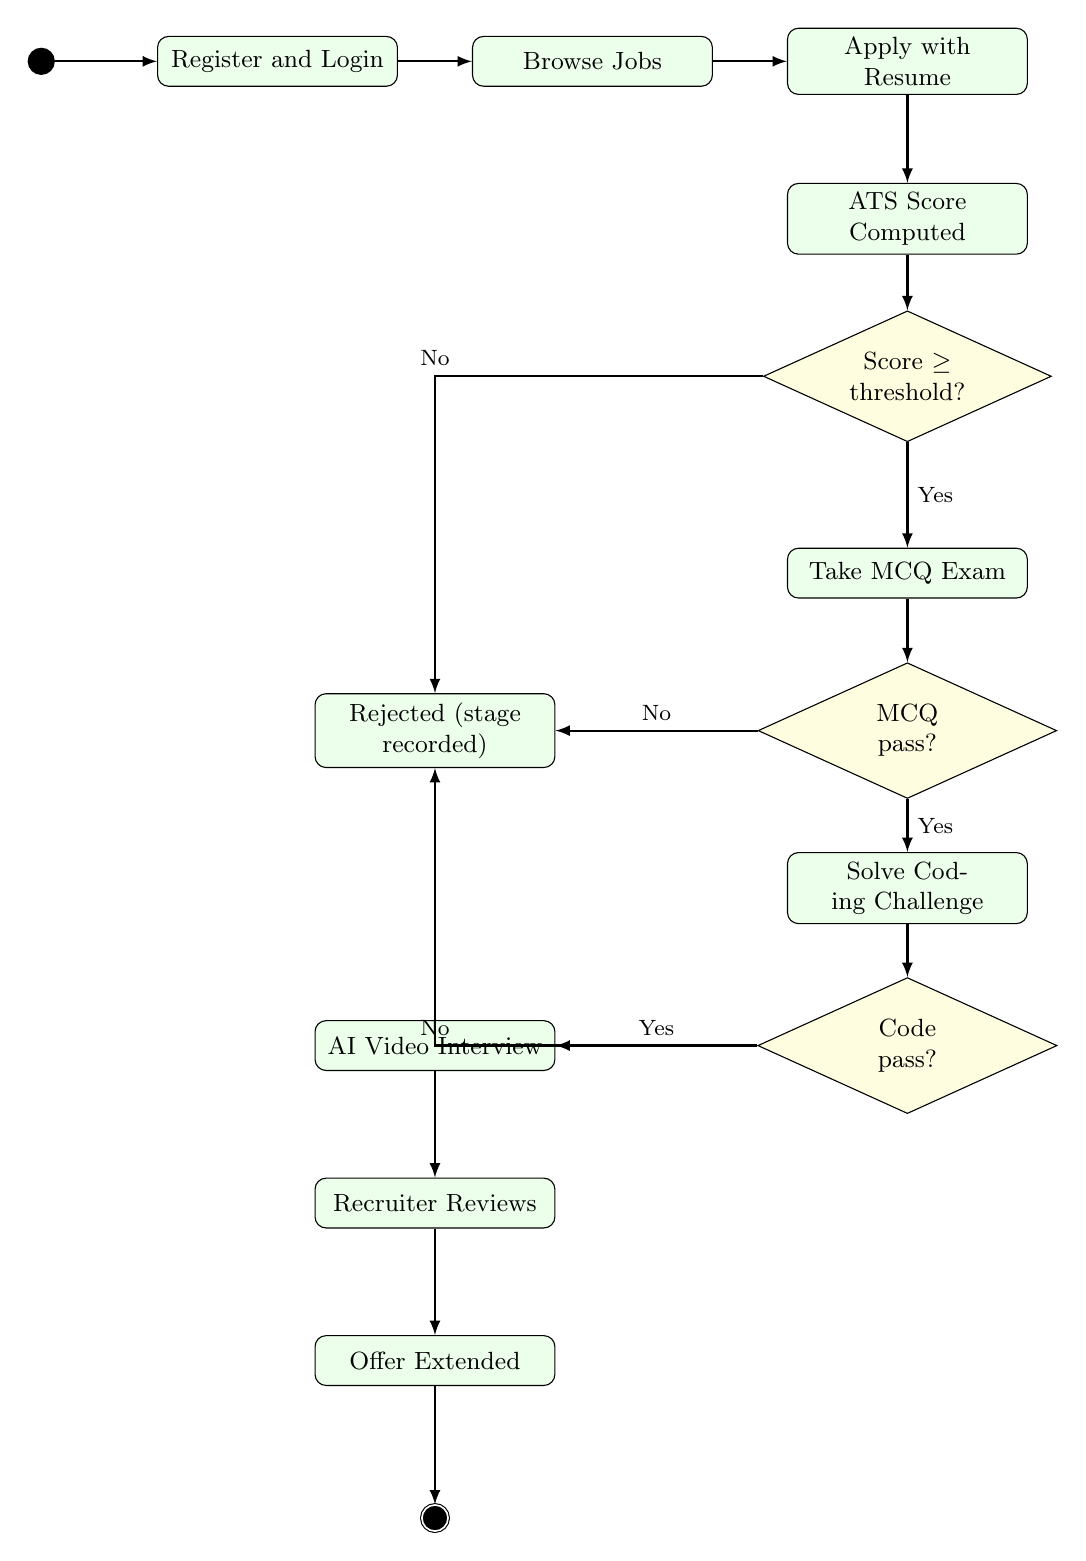
\begin{tikzpicture}[
  start/.style={circle, draw, fill=black, minimum size=0.3cm},
  stop/.style={circle, draw, fill=black, minimum size=0.3cm, double},
  action/.style={rectangle, draw, rounded corners, fill=green!8, text width=8em, text centered, minimum height=1.8em, font=\small},
  decision/.style={diamond, draw, fill=yellow!12, text width=4.5em, text centered, aspect=2.2, font=\small},
  arrow/.style={-latex, thick}
]
  \node[start]    (s)  at (0,0) {};
  \node[action]   (a1) at (3,0) {Register and Login};
  \node[action]   (a2) at (7,0) {Browse Jobs};
  \node[action]   (a3) at (11,0) {Apply with Resume};
  \node[action]   (a4) at (11,-2) {ATS Score Computed};
  \node[decision] (d1) at (11,-4) {Score $\geq$ threshold?};
  \node[action]   (a5) at (11,-6.5) {Take MCQ Exam};
  \node[decision] (d2) at (11,-8.5) {MCQ pass?};
  \node[action]   (a6) at (11,-10.5) {Solve Coding Challenge};
  \node[decision] (d3) at (11,-12.5) {Code pass?};
  \node[action]   (a7) at (5,-12.5) {AI Video Interview};
  \node[action]   (a8) at (5,-14.5) {Recruiter Reviews};
  \node[action]   (a9) at (5,-16.5) {Offer Extended};
  \node[action]   (rej) at (5,-8.5) {Rejected (stage recorded)};
  \node[stop]     (e)  at (5,-18.5) {};

  \draw[arrow] (s) -- (a1);
  \draw[arrow] (a1) -- (a2);
  \draw[arrow] (a2) -- (a3);
  \draw[arrow] (a3) -- (a4);
  \draw[arrow] (a4) -- (d1);
  \draw[arrow] (d1) -- node[right, font=\footnotesize]{Yes} (a5);
  \draw[arrow] (d1) -| node[above, font=\footnotesize]{No} (rej);
  \draw[arrow] (a5) -- (d2);
  \draw[arrow] (d2) -- node[right, font=\footnotesize]{Yes} (a6);
  \draw[arrow] (d2) -- node[above, font=\footnotesize]{No} (rej);
  \draw[arrow] (a6) -- (d3);
  \draw[arrow] (d3) -- node[above, font=\footnotesize]{Yes} (a7);
  \draw[arrow] (d3) -| node[above, font=\footnotesize]{No} (rej);
  \draw[arrow] (a7) -- (a8);
  \draw[arrow] (a8) -- (a9);
  \draw[arrow] (a9) -- (e);
\end{tikzpicture}
}
\caption{Activity diagram for the candidate application lifecycle}
\label{fig:activity}
\end{figure}

The activity diagram reveals the sequential, gate-keeping nature of SmartHire's evaluation pipeline. Each stage produces a quantitative score, and advancement requires meeting a configurable threshold. This design ensures that only candidates who demonstrate competence at each level proceed to the next, reducing the evaluation burden on later (more expensive) stages such as coding challenges and video interviews. When a candidate is rejected, the specific stage at which the rejection occurred is recorded, enabling the transparent feedback mechanism described in Chapter~1.

\section{Complete SmartHire Recruitment Workflow}
\label{sec:complete-workflow}

This section presents the end-to-end workflow that ties together all system components, from job posting creation by a recruiter to the final hiring decision.

\begin{enumerate}[leftmargin=1.5em]
  \item \textbf{Job Posting}: A recruiter creates a job posting in draft status, specifying the title, description, required skills, location, salary range, and employment type. The recruiter publishes the job when ready, making it visible on the candidate portal.

  \item \textbf{Candidate Application}: A candidate discovers the job listing, reviews the description, and applies by uploading their PDF resume. The system immediately triggers the ATS scoring pipeline.

  \item \textbf{ATS Screening}: The resume text is extracted, parsed, and evaluated against the job requirements via the Gemini API. The resulting score (0--10) is stored with the application. Candidates above the threshold advance; those below receive a rejection notification with their score.

  \item \textbf{MCQ Assessment}: Qualifying candidates are invited to complete a timed MCQ examination. Questions are drawn from the job's question pool and presented in randomised order. The timer enforces auto-submission. Scores are computed and stored instantly.

  \item \textbf{Coding Challenge}: Candidates who pass the MCQ stage are presented with coding problems in the Monaco IDE. They write solutions, run them against sample test cases, and submit for evaluation against the hidden test suite. The percentage of passing tests determines their coding score.

  \item \textbf{AI Video Interview}: Qualifying candidates enter the video interview room, where they respond to structured questions while being recorded. Transcriptions are sent to Gemini for evaluation, producing a detailed scorecard.

  \item \textbf{Recruiter Review}: The recruiter reviews the candidate's complete evaluation profile on the Kanban board: ATS score, MCQ score, coding score, and AI interview scorecard. Based on this data, the recruiter decides to advance, reject, or schedule a follow-up.

  \item \textbf{Offer Generation}: For selected candidates, the recruiter generates a customised PDF offer letter specifying salary, position, joining date, and terms. The offer is sent through the platform.

  \item \textbf{Candidate Response}: The candidate views the offer on their portal and accepts or declines. The response updates the application status and the recruiter's pipeline board.
\end{enumerate}

\section{Module Interaction Matrix}
\label{sec:module-interaction}

Table~\ref{tab:module-matrix} documents the dependencies between SmartHire's principal modules. Each cell indicates whether the row module invokes or depends on the column module during normal operation.

\begin{table}[htbp]
\centering
\caption{Module interaction matrix}
\label{tab:module-matrix}
\small
\begin{tabular}{l|cccccc}
\toprule
 & \rotatebox{60}{\textbf{Auth}} & \rotatebox{60}{\textbf{Job Mgmt}} & \rotatebox{60}{\textbf{ATS}} & \rotatebox{60}{\textbf{Assessment}} & \rotatebox{60}{\textbf{Interview}} & \rotatebox{60}{\textbf{Offer}} \\
\midrule
Auth        & ---          & ---          & ---          & ---          & ---          & ---          \\
Job Mgmt    & \checkmark   & ---          & ---          & ---          & ---          & ---          \\
ATS         & \checkmark   & \checkmark   & ---          & ---          & ---          & ---          \\
Assessment  & \checkmark   & \checkmark   & \checkmark   & ---          & ---          & ---          \\
Interview   & \checkmark   & \checkmark   & ---          & \checkmark   & ---          & ---          \\
Offer       & \checkmark   & \checkmark   & ---          & ---          & ---          & ---          \\
\bottomrule
\end{tabular}
\end{table}

The matrix confirms that the authentication module is a universal dependency, as every operation requires identity verification. The ATS and assessment modules depend on job management for retrieving job specifications and question pools. The interview module depends on the assessment module to verify that the candidate has completed prior stages before being allowed to proceed.

\section{API Request-Response Lifecycle}
\label{sec:api-lifecycle}

Every API request in SmartHire follows a standardised lifecycle through five processing phases:

\begin{enumerate}[leftmargin=1.5em]
  \item \textbf{Authentication}: The middleware extracts the JWT from the request cookie, verifies its signature and expiration using Supabase's \texttt{getUser()} method, and attaches the authenticated user object to the request context. Unauthenticated requests receive a 401 response.

  \item \textbf{Authorisation}: The route handler checks whether the authenticated user has the required role (candidate, recruiter, or admin) for the requested operation. Requests from users with insufficient privileges receive a 403 response.

  \item \textbf{Validation}: Request body parameters are validated against predefined schemas using runtime validation. Malformed requests receive a 400 response with descriptive error messages.

  \item \textbf{Business Logic}: The validated request is processed by the appropriate service module, which may involve database queries, external API calls (Gemini), file operations (Supabase Storage), or a combination thereof.

  \item \textbf{Response}: The result is serialised to JSON and returned with an appropriate HTTP status code (200 for success, 201 for resource creation, 400/401/403/404/500 for various error conditions).
\end{enumerate}

This standardised lifecycle ensures consistent error handling, security enforcement, and response formatting across all endpoints.


\makechaptertitlepage{5}{IMPLEMENTATION}
\setcounter{chapter}{4}
\chapter{Implementation}
\label{ch:implementation}

This chapter documents the implementation of each major module in SmartHire, covering purpose, workflow, key design decisions, code-level details, and integration with the rest of the system. Code excerpts are drawn from the actual source repository and are annotated with explanatory commentary.

\section{Project Structure}
\label{sec:project-structure}

SmartHire is organised as a monorepo managed by pnpm workspaces. The primary application lives in \texttt{apps/web/} and follows Next.js~15's App Router conventions. Application code is further subdivided using route groups:

\begin{lstlisting}[caption={Top-level directory layout}, language={}]
apps/web/src/
  app/
    (auth)/          # Login, registration
    (candidate)/     # Candidate portal routes
    (recruiter)/     # Recruiter portal routes
    (admin)/         # Admin dashboard
    (public)/        # Public pages (job listings)
    api/             # Backend API routes
  services/          # Business logic layer
  utils/             # Shared utilities
  components/        # Reusable UI components
\end{lstlisting}

The \texttt{services/} directory contains the business logic, separated into domain-specific files: \texttt{auth.ts}, \texttt{job-service.ts}, \texttt{candidate-service.ts}, \texttt{application-service.ts}, \texttt{resume-service.ts}, and subdirectories for \texttt{assessment/}, \texttt{interview/}, \texttt{ai/}, \texttt{analytics/}, and \texttt{notification/}. Each service file encapsulates data access patterns and business rules for its domain, keeping API route handlers thin.

\section{Module 1: Authentication and Session Management}
\label{sec:impl-auth}

\begin{figure}[H]
  \centering
  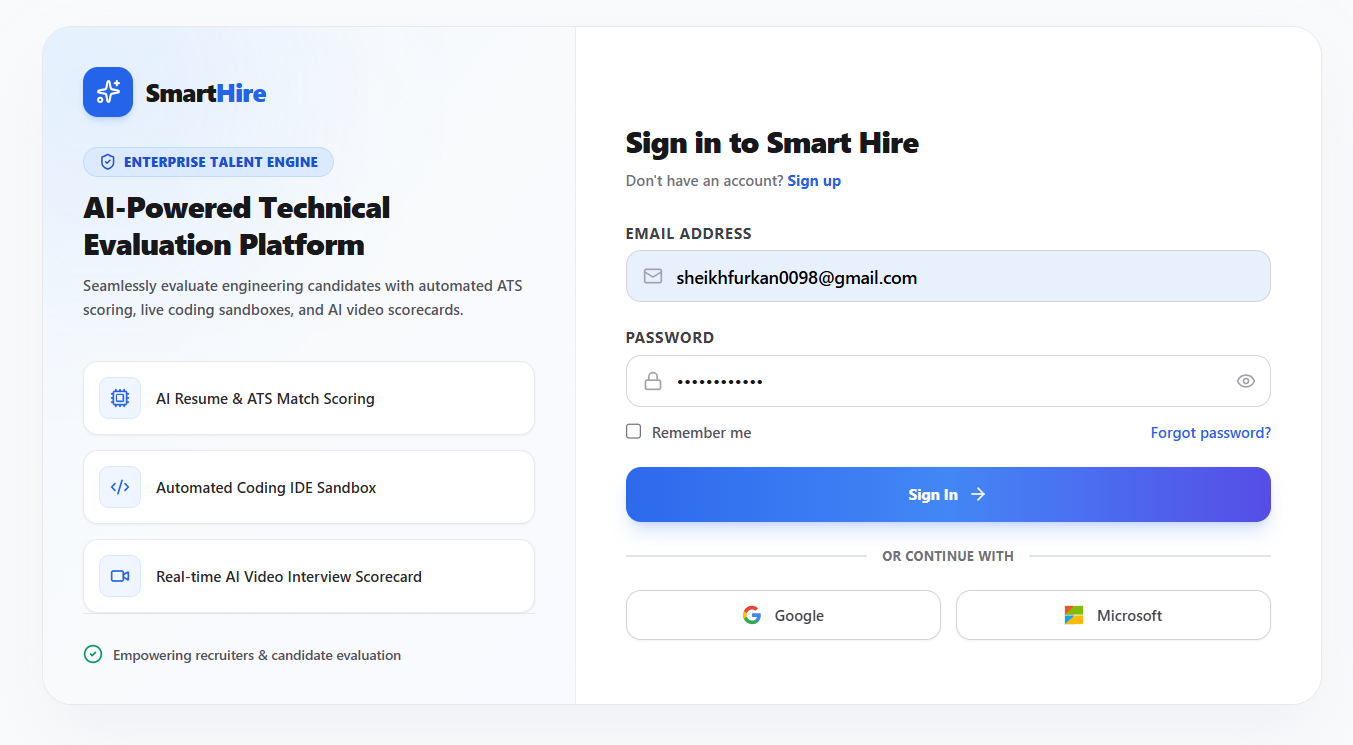
\includegraphics[width=0.85\textwidth]{images/login and registration interface.png}
  \caption{Login and registration interface}
  \label{fig:login_register}
\end{figure}

\subsection{Purpose}

The authentication module handles user registration, login, session token management, and role-based access control. It must distinguish between three user roles (candidate, recruiter, administrator) and route each user to the appropriate portal upon successful authentication.

\subsection{Implementation Details}

Authentication is delegated to Supabase Auth, which provides email/password registration, JWT token issuance, and session refresh. A critical implementation detail is the browser client singleton pattern. In a Next.js application, components may re-render frequently during hydration; creating a new Supabase client on each render would produce redundant network connections and potential race conditions. The singleton ensures that only one client instance exists per browser tab.

\begin{lstlisting}[language=Java, caption={Supabase browser client singleton}]
// apps/web/src/utils/supabase/client.ts
import { createBrowserClient } from "@supabase/ssr";

let browserClient: ReturnType<typeof createBrowserClient> | null
  = null;

export function getSupabaseBrowserClient() {
  if (typeof window === "undefined") {
    // SSR: create a fresh client per request
    return createBrowserClient(
      process.env.NEXT_PUBLIC_SUPABASE_URL!,
      process.env.NEXT_PUBLIC_SUPABASE_ANON_KEY!
    );
  }
  if (!browserClient) {
    browserClient = createBrowserClient(
      process.env.NEXT_PUBLIC_SUPABASE_URL!,
      process.env.NEXT_PUBLIC_SUPABASE_ANON_KEY!
    );
  }
  return browserClient;
}
\end{lstlisting}

The conditional check on \texttt{typeof window} ensures that server-side rendering (where \texttt{window} is undefined) always creates a fresh client, avoiding stale session data across different server requests.

\subsection{Security Considerations}

Passwords are hashed by Supabase using bcrypt with a configurable cost factor. JWT tokens are stored in HTTP-only cookies to prevent cross-site scripting (XSS) attacks from accessing them. API routes validate the JWT on every request using Supabase's \texttt{getUser()} method, which verifies the token signature and checks expiration.

\section{Module 2: Job Management}
\label{sec:impl-jobs}

\begin{figure}[H]
  \centering
  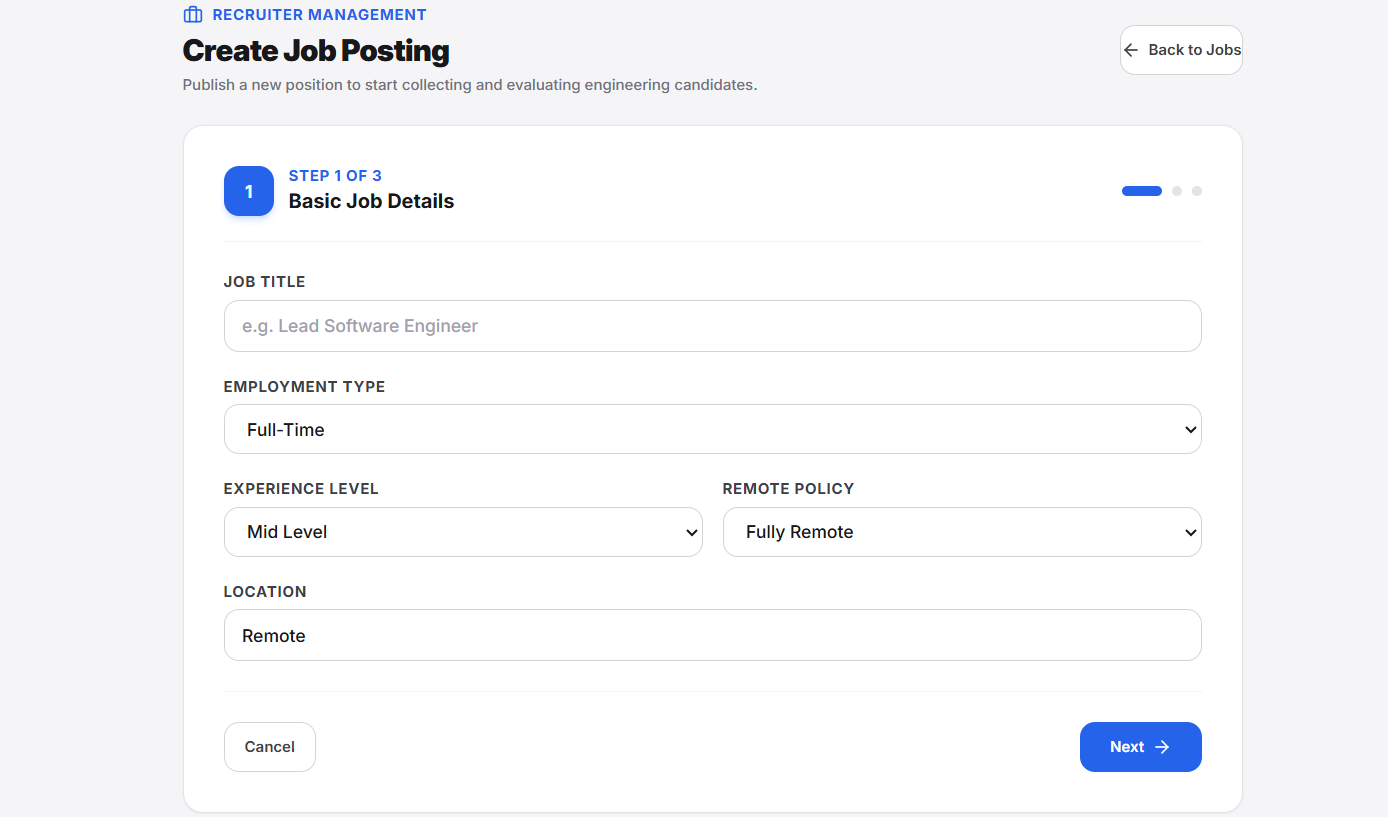
\includegraphics[width=0.85\textwidth]{images/job creation interface.png}
  \caption{Job creation wizard interface showcasing light mode theme and multi-step positioning parameters.}
  \label{fig:job_creation}
\end{figure}

\subsection{Purpose}

The job management module allows recruiters to create, edit, publish, and close job postings. Each job posting specifies a title, description, required skills, location, employment type, salary range, and a status field that governs visibility to candidates.

\subsection{Workflow}

Jobs follow a simple lifecycle: \textbf{Draft} $\rightarrow$ \textbf{Published} $\rightarrow$ \textbf{Closed}. A newly created job defaults to draft status and is not visible on the candidate portal. When the recruiter publishes the job, it appears in the public job directory. Closing a job removes it from the directory and prevents new applications.

\subsection{Database Interaction}

The job service (\texttt{job-service.ts}) exposes methods for creating, retrieving, updating, and listing jobs. All queries are scoped to the authenticated recruiter's company to enforce multi-tenant isolation:

\begin{lstlisting}[language=Java, caption={Job retrieval scoped to recruiter's company}]
async function getJobsByRecruiter(recruiterId: string) {
  const { data, error } = await supabase
    .from("job.jobs")
    .select("*")
    .eq("recruiter_id", recruiterId)
    .order("created_at", { ascending: false });
  if (error) throw error;
  return data;
}
\end{lstlisting}

\section{Module 3: Candidate Profile and Job Directory}
\label{sec:impl-candidate}

\begin{figure}[H]
  \centering
  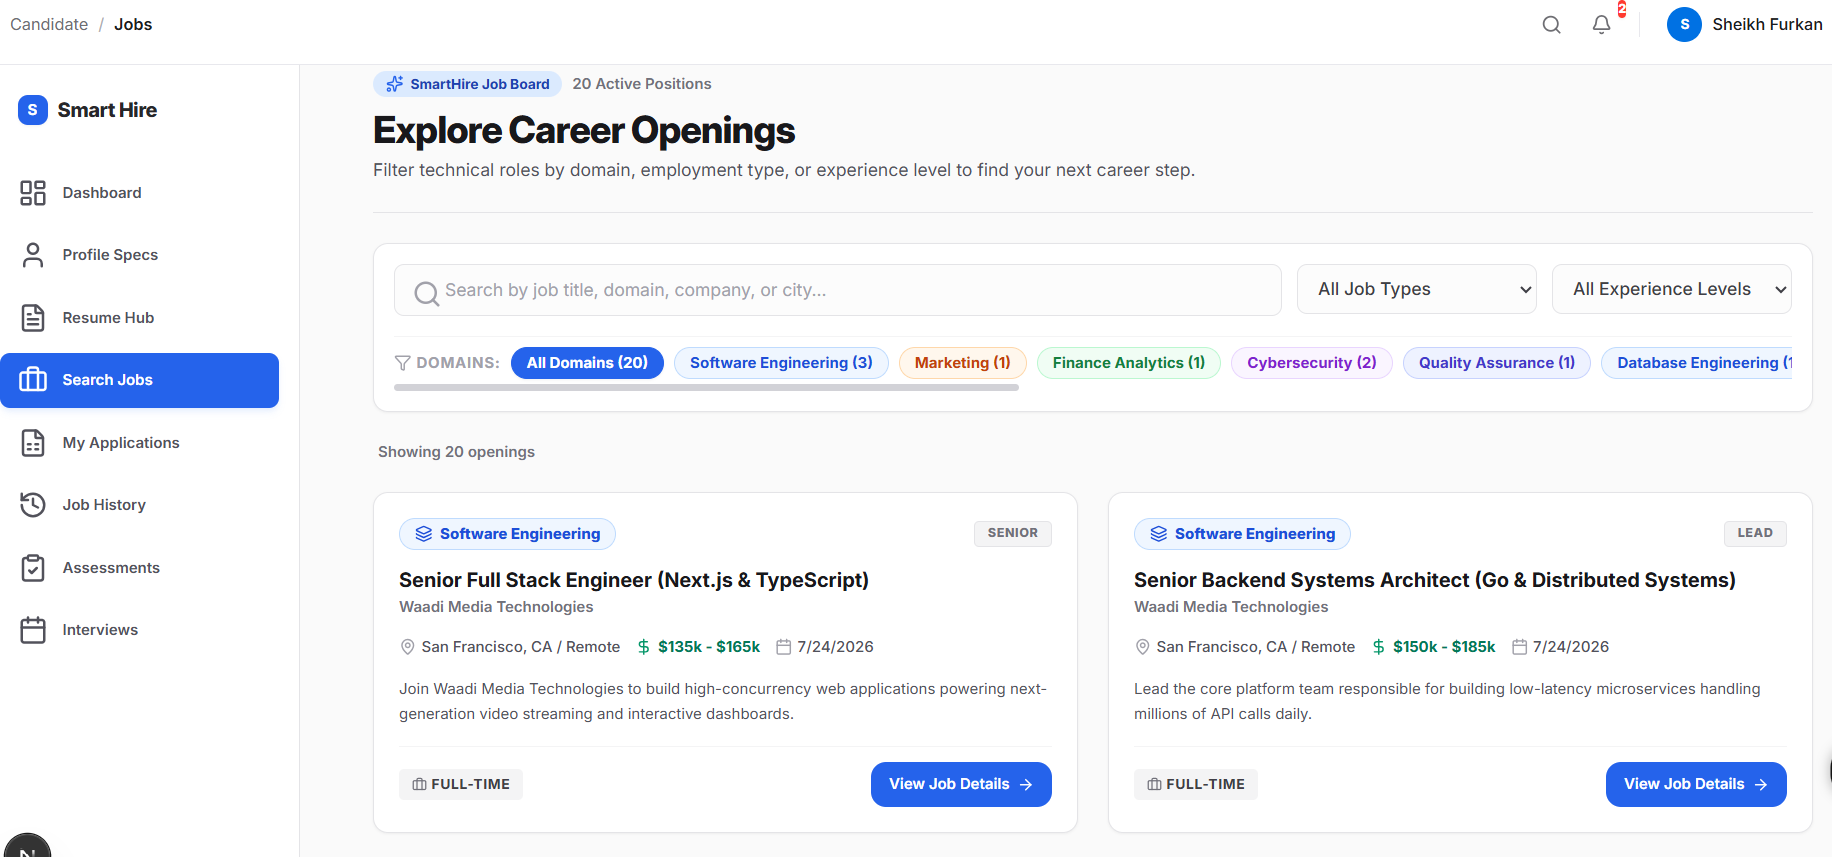
\includegraphics[width=0.85\textwidth]{images/candidate job dirwithsearchfilters.png}
  \caption{Candidate job directory with search filters}
  \label{fig:candidate_job_directory}
\end{figure}

\begin{figure}[H]
  \centering
  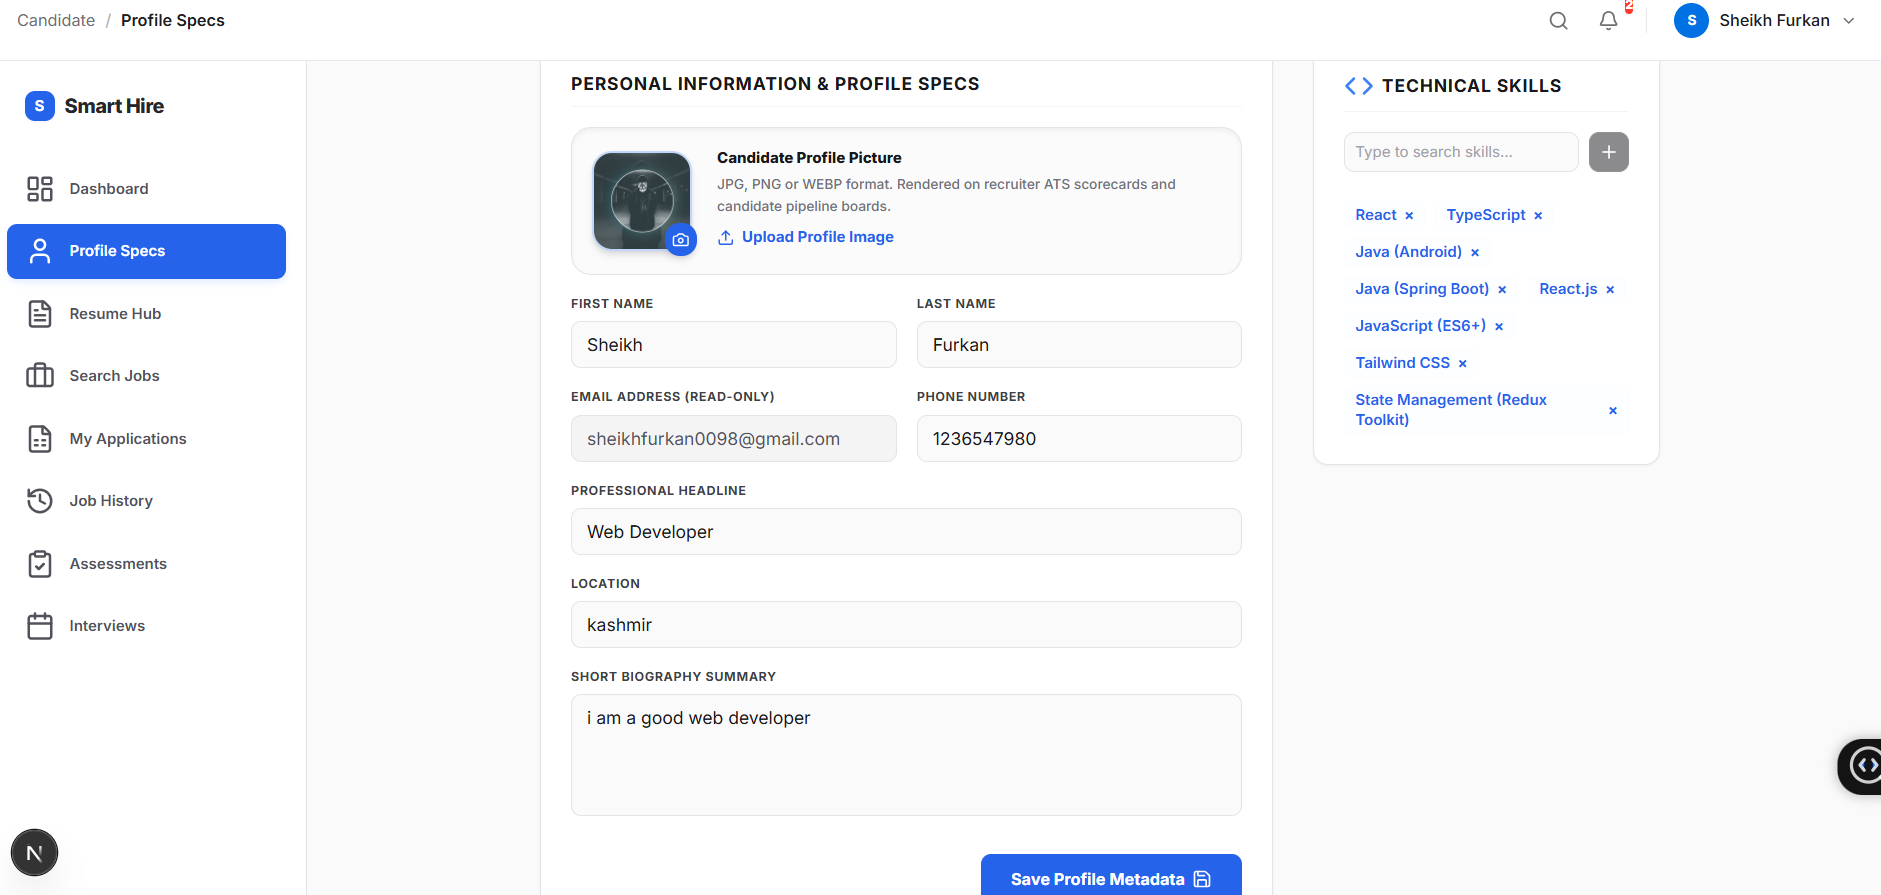
\includegraphics[width=0.85\textwidth]{images/candidate profile editor.png}
  \caption{Candidate profile editor interface}
  \label{fig:candidate_profile_editor}
\end{figure}

\subsection{Purpose}

Candidates need a profile that stores their personal information, skills, education, and work experience. They also need to browse and search published job listings.

\subsection{Implementation Details}

The candidate profile is pre-populated from Supabase Auth metadata (name, email) upon first login, reducing manual data entry. Additional fields (phone, skills array, experience years) are stored in the \texttt{candidate.candidates} table. The job directory page fetches all published jobs using a filtered query and presents them in a searchable, paginated grid. Candidates can filter by keyword, location, job category, and employment type.

\section{Module 4: Resume Upload and ATS Scoring}
\label{sec:impl-ats}

\begin{figure}[H]
  \centering
  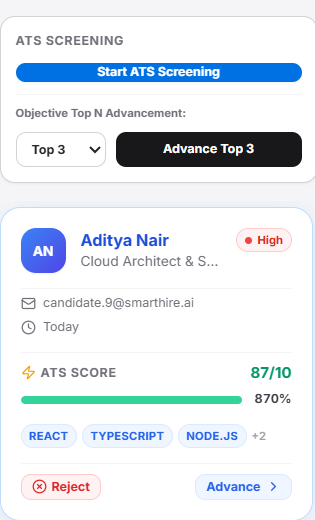
\includegraphics[width=0.65\textwidth]{images/ats view.png}
  \caption{ATS Board}
  \label{fig:ats_board}
\end{figure}

\subsection{Purpose}

When a candidate applies for a job, the system must extract text from the uploaded PDF resume, parse it into structured fields, and compute a relevance score against the job description.

\subsection{Workflow}

\begin{enumerate}[leftmargin=1.5em]
  \item The candidate selects a PDF file and submits the application form.
  \item The frontend uploads the file to Supabase Storage and sends the file URL along with the application data to the API.
  \item The resume service extracts text from the PDF using a server-side parsing library.
  \item The extracted text and the job description are sent to the Gemini API with a structured prompt requesting a relevance score on a 0--10 scale, along with dimensional breakdowns.
  \item The API response is parsed, validated, and stored in the application record.
\end{enumerate}

\section{Module 5: MCQ Assessment Engine}
\label{sec:impl-mcq}

\begin{figure}[H]
  \centering
  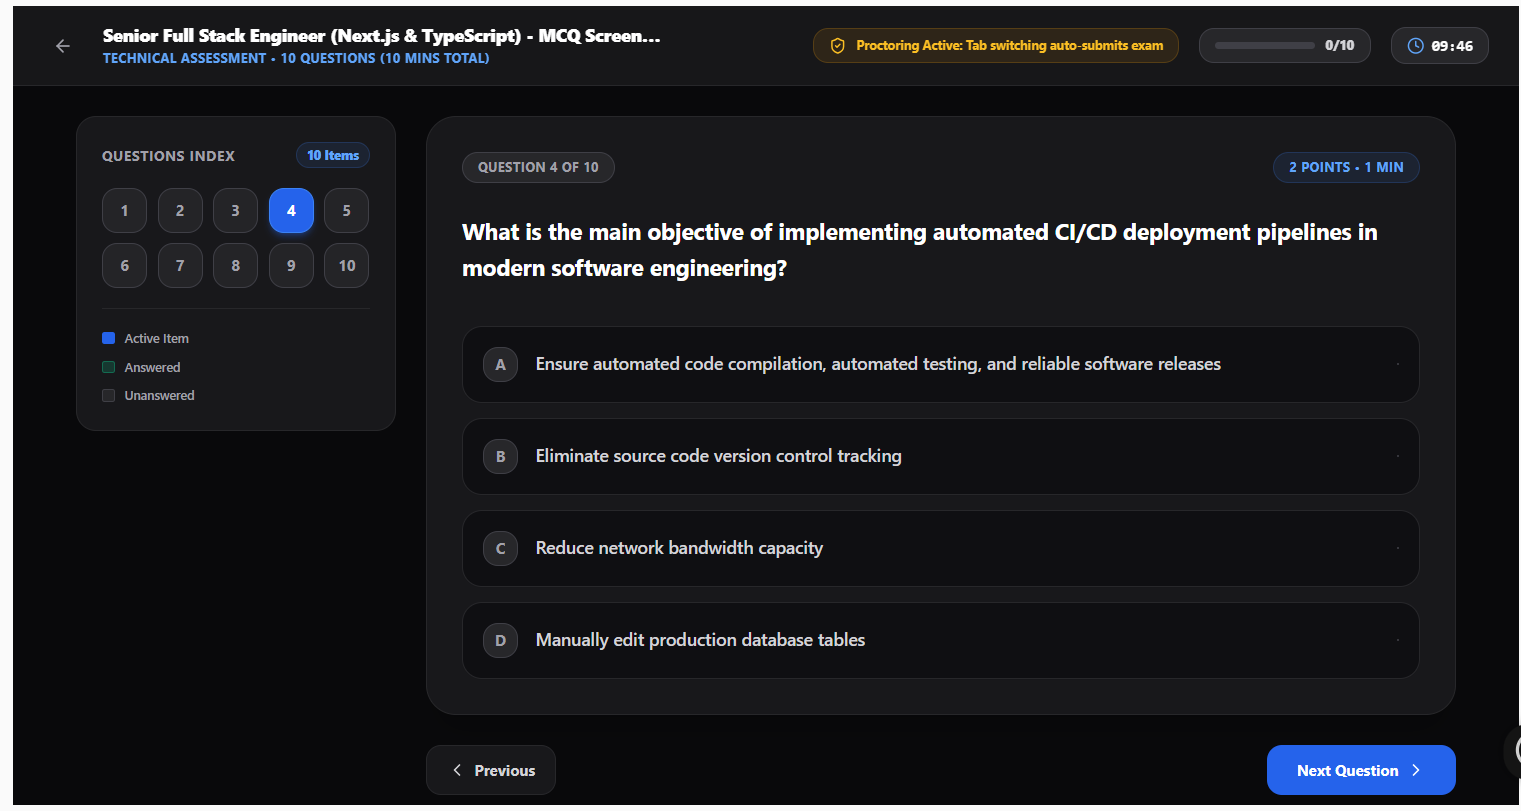
\includegraphics[width=0.85\textwidth]{images/mcq.png}
  \caption{MCQ examination interface with countdown timer}
  \label{fig:mcq_exam}
\end{figure}

\subsection{Purpose}

The MCQ engine administers timed multiple-choice assessments to candidates who pass the ATS screening threshold. It must enforce time limits, randomise question order to reduce cheating, auto-submit when the timer expires, and compute scores instantly.

\subsection{Implementation Details}

Each job can have an associated question pool stored in the \texttt{assessment.questions} table. When a candidate begins an MCQ assessment, the system creates an attempt record in \texttt{assessment.attempts}, selects questions from the pool, randomises their order, and starts a client-side countdown timer. The timer is implemented using React's \texttt{useEffect} hook with a one-second interval. If the timer reaches zero before the candidate manually submits, the system automatically submits all recorded answers.

Score computation is straightforward: the number of correct answers divided by the total number of questions, multiplied by 100. The computed score is stored in the application record.

\section{Module 6: Interactive Coding Assessment}
\label{sec:impl-coding}

\begin{figure}[H]
  \centering
  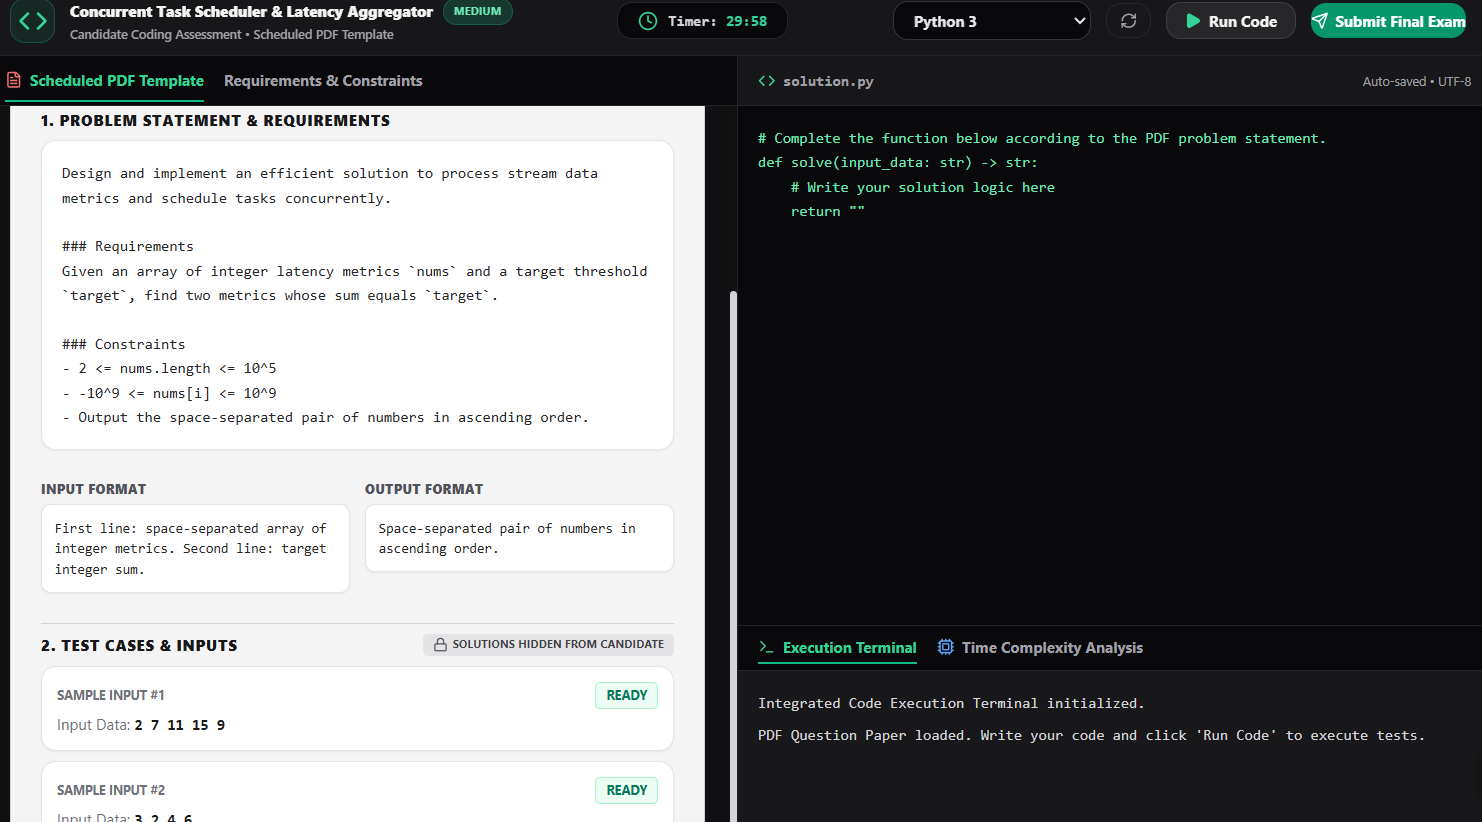
\includegraphics[width=0.85\textwidth]{images/coding round.png}
  \caption{coding round ide}
  \label{fig:coding_ide}
\end{figure}

\subsection{Purpose}

The coding module provides a browser-based IDE where candidates write and execute code to solve programming challenges. It replaces the need for a separate coding assessment platform.

\subsection{Implementation Details}

The code editor is built using \texttt{@monaco-editor/react}, which embeds the same editing engine used by Visual Studio Code. The editor supports syntax highlighting, auto-indentation, and bracket matching for JavaScript and Python. When the candidate clicks ``Run,'' the code is sent to a server-side API endpoint that executes it in a sandboxed environment, captures the output, and compares it against expected results for each test case.

Each test case specifies an input string and an expected output string. The execution environment runs the candidate's code with the input piped to stdin, captures stdout, and performs a string comparison. Test results are returned to the frontend, showing pass/fail status for each test case. The final score is the percentage of test cases passed.

\section{Module 7: AI Video Interview}
\label{sec:impl-interview}

\begin{figure}[H]
  \centering
  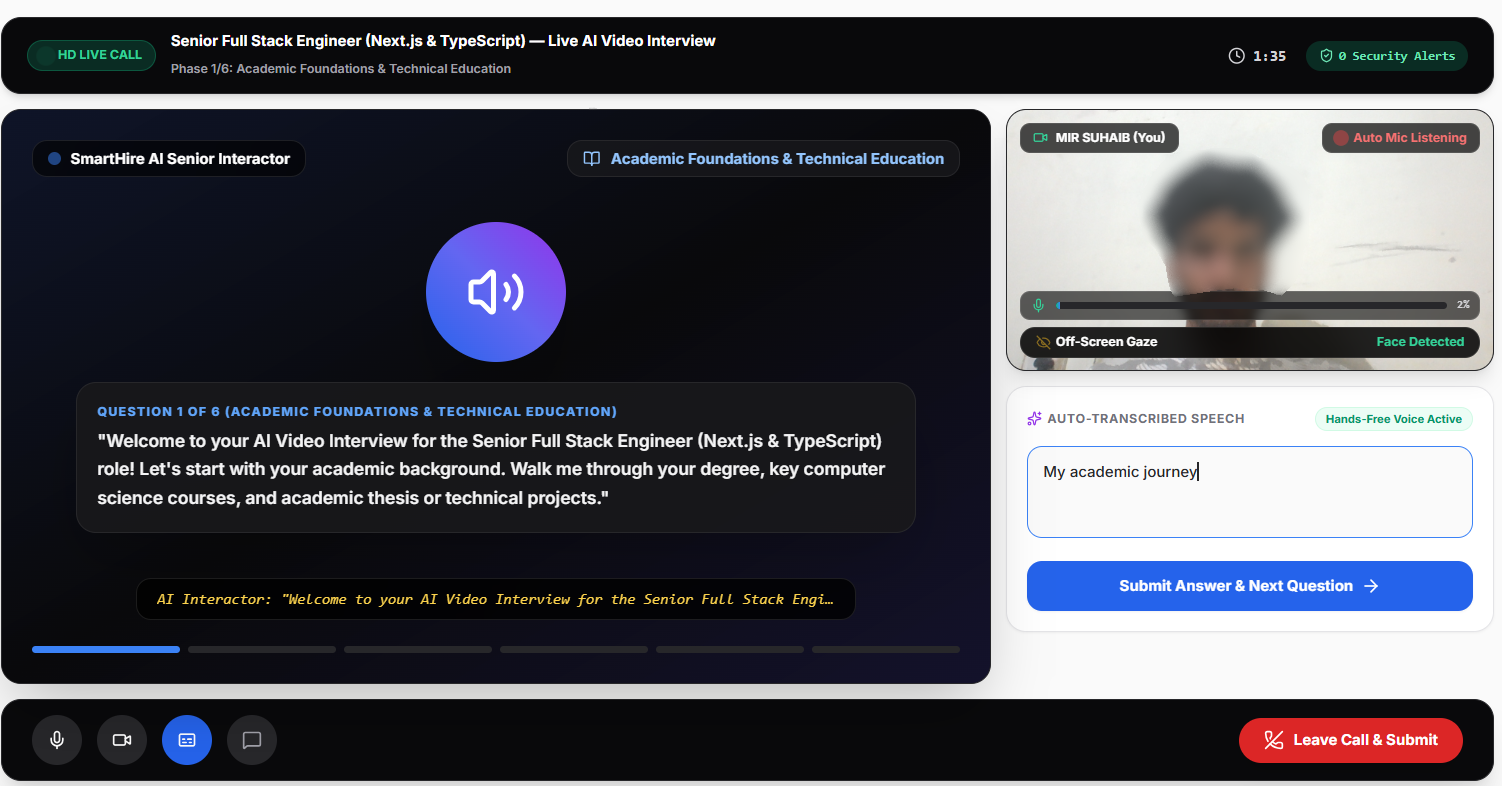
\includegraphics[width=0.85\textwidth]{images/ai interview.png}
  \caption{Live AI video interview recording room with real-time audio transcript, proctoring gaze detection, and voice evaluation.}
  \label{fig:ai_interview}
\end{figure}

\subsection{Purpose}

The video interview module enables asynchronous, AI-evaluated interviews. Candidates record responses to predefined questions, and the system uses the Gemini API to evaluate the quality of their answers.

\subsection{Implementation Details}

The interview interface presents questions one at a time. For each question, the candidate clicks ``Record,'' speaks their response while being recorded via the browser's MediaRecorder API, and clicks ``Stop'' when finished. The recorded audio is transcribed (either client-side using the Web Speech API or server-side using a transcription service) and stored alongside the question in a structured format.

Once all questions have been answered, the complete set of question-response pairs is sent to the Gemini API with an evaluation prompt. The prompt instructs the model to assess each response across four dimensions: \textit{technical knowledge}, \textit{communication clarity}, \textit{problem-solving approach}, and \textit{depth of reasoning}. The model returns a structured JSON scorecard with per-dimension ratings and an overall recommendation.

\subsection{Scorecard Categories}

The overall recommendation uses a five-point scale:

\begin{table}[htbp]
\centering
\caption{AI interview scorecard recommendation categories}
\label{tab:scorecard}
\small
\begin{tabular}{lp{4in}}
\toprule
\textbf{Category} & \textbf{Interpretation} \\
\midrule
\texttt{strong\_hire}    & Exceptional responses; candidate demonstrates deep expertise and clear communication. \\
\texttt{hire}            & Solid responses; candidate meets or exceeds expectations. \\
\texttt{neutral}         & Adequate responses; further evaluation may be warranted. \\
\texttt{no\_hire}         & Below expectations; significant gaps in knowledge or communication. \\
\texttt{strong\_no\_hire}  & Poor responses; candidate does not meet minimum requirements. \\
\bottomrule
\end{tabular}
\end{table}

\section{Module 8: Recruiter Kanban Pipeline}
\label{sec:impl-kanban}

\begin{figure}[H]
  \centering
  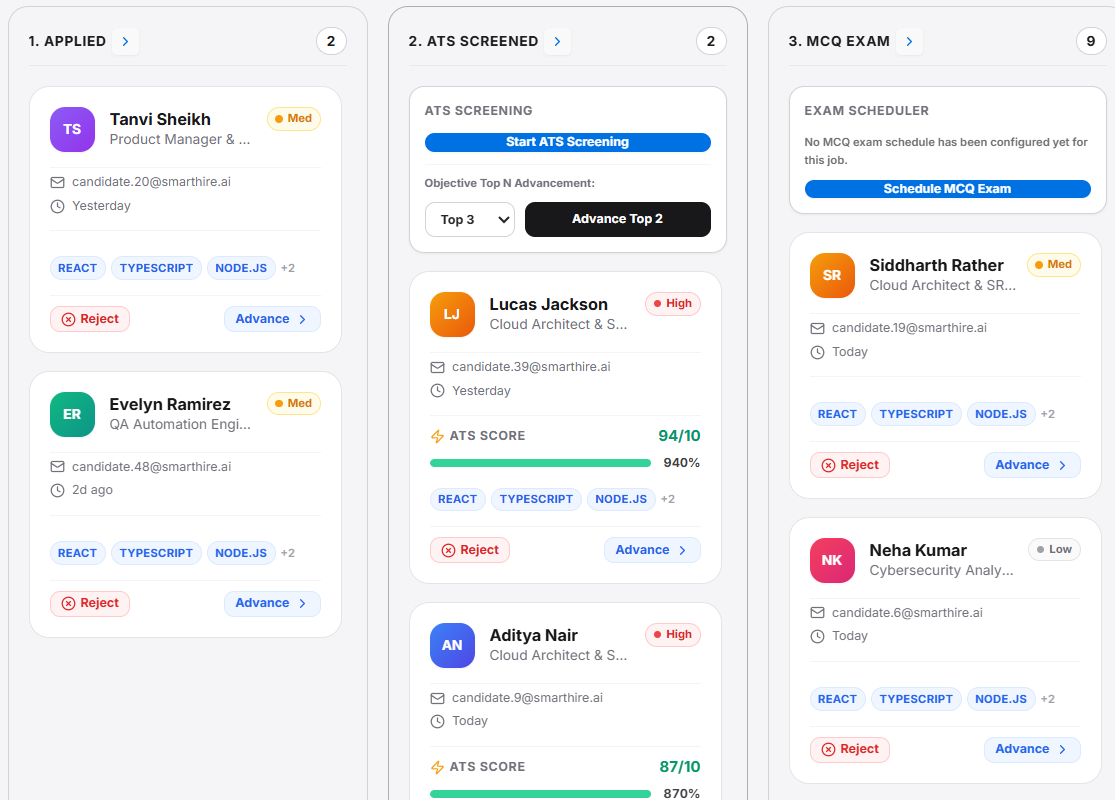
\includegraphics[width=0.85\textwidth]{images/kanban board.png}
  \caption{Recruiter Kanban pipeline board showing multi-stage candidate progression and automated ATS screening controls.}
  \label{fig:pipeline_board}
\end{figure}

\subsection{Purpose}

The Kanban board gives recruiters a visual overview of all candidates for a given job, organised by pipeline stage. It supports drag-and-drop stage transitions, real-time status updates, and stage-specific rejection tracking.

\subsection{Implementation Details}

The Kanban board is implemented as a client-side React component that fetches all applications for the selected job and groups them into columns by stage. Each column represents a pipeline stage: Applied, ATS Screened, MCQ, Coding, Interview, Offer, and Hired. Dragging a card from one column to another triggers an API call that updates the application's stage in the database.

Stage transitions are validated on the server to ensure they follow the prescribed order. If a recruiter moves a candidate to a rejected state, the system records which stage the rejection occurred at and optionally logs a rejection reason. This information is surfaced on the candidate's application history page.

\section{Module 9: Recruiter Dashboard}
\label{sec:impl-dashboard}

\begin{figure}[H]
  \centering
  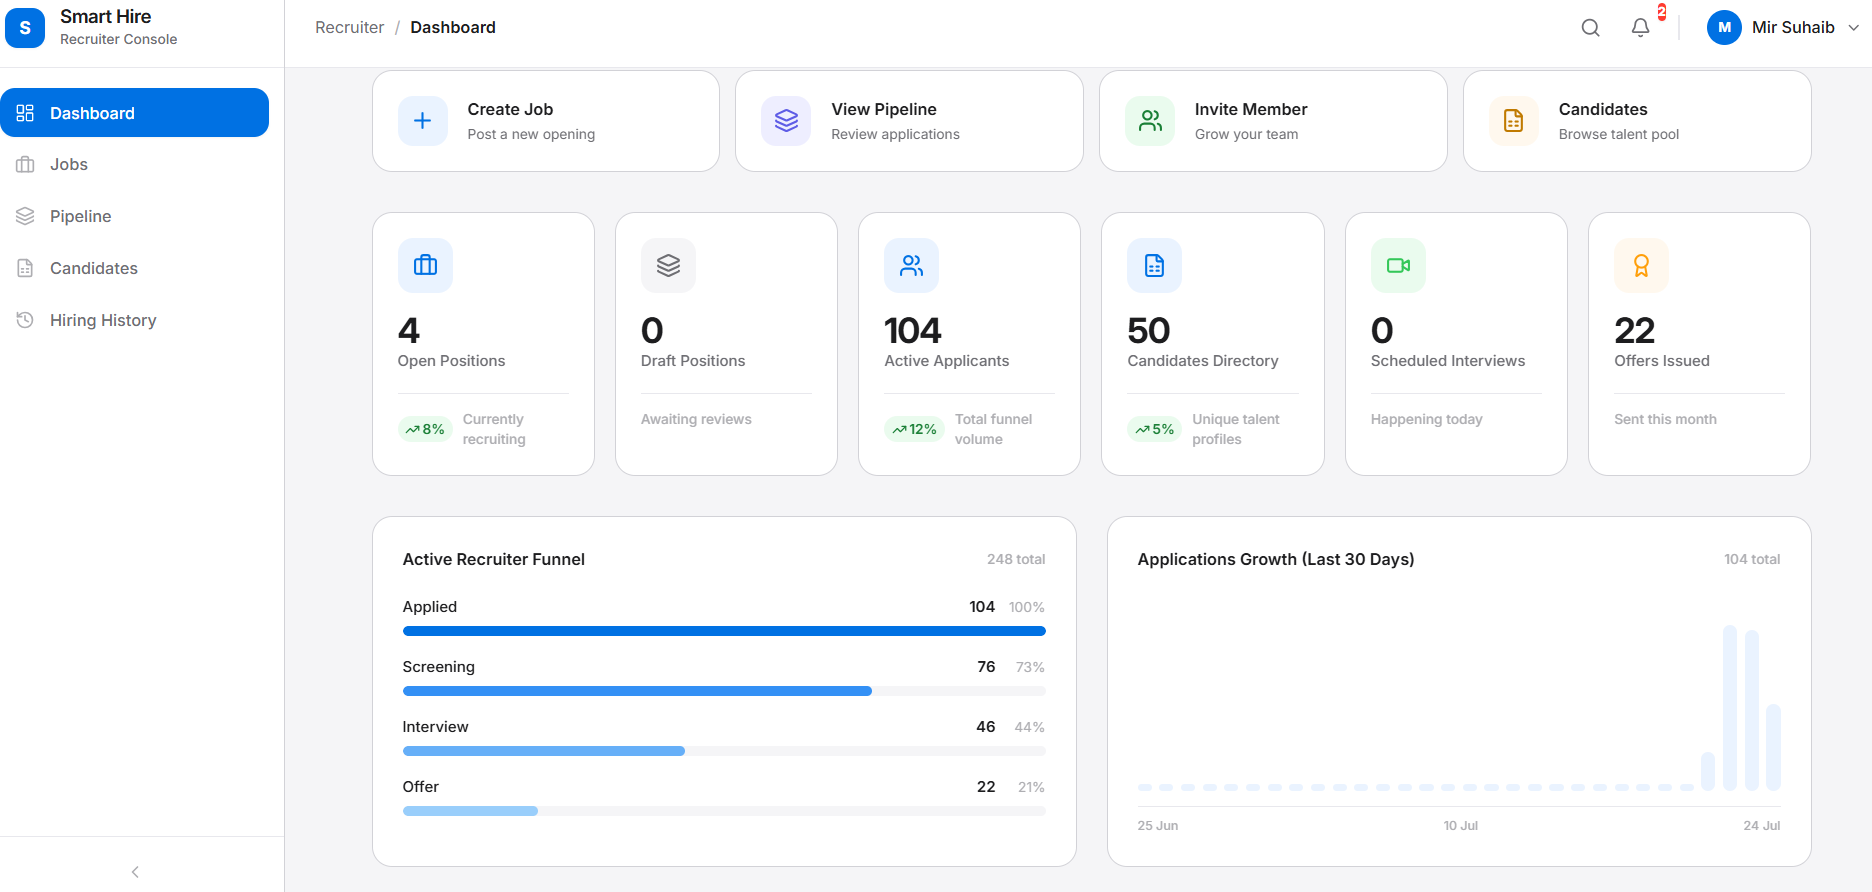
\includegraphics[width=0.85\textwidth]{images/recruiter dasboard with hiring metrics.png}
  \caption{Recruiter dashboard displaying real-time hiring funnel metrics, active applicant counts, and application growth analytics.}
  \label{fig:recruiter_dashboard}
\end{figure}

\subsection{Purpose}

The dashboard provides recruiters with at-a-glance metrics on their hiring activity: open positions, active applicants, interviews scheduled, offers issued, and pipeline funnel analytics.

\subsection{Multi-Tenant Scoping}

A critical design requirement is that each recruiter sees only metrics related to their own job postings. The dashboard queries are scoped by joining the \texttt{application.applications} table against the \texttt{job.jobs} table where the \texttt{recruiter\_id} matches the authenticated user. This prevents data from other recruiters (even within the same company) from leaking into the dashboard view.

\section{Module 10: Offer Letter Generation}
\label{sec:impl-offer}

\begin{figure}[H]
  \centering
  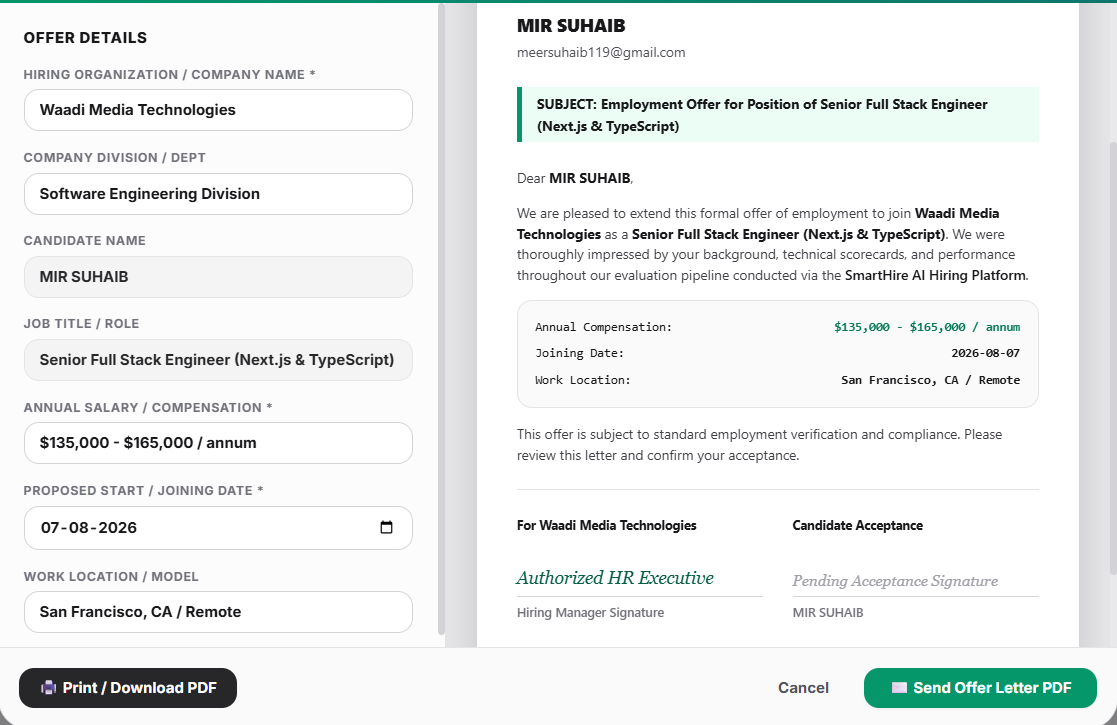
\includegraphics[width=0.85\textwidth]{images/offerletter.png}
  \caption{Official offer letter generator interface with real-time PDF preview and signature workflow.}
  \label{fig:offer_letter}
\end{figure}

\subsection{Purpose}

Once a recruiter decides to hire a candidate, the system generates a formal PDF offer letter that can be customised, previewed, and dispatched to the candidate.

\subsection{Implementation Details}

Offer letters are generated client-side using the jsPDF library combined with html2canvas for rendering styled HTML templates into PDF format. The recruiter fills in a form specifying salary, joining date, position title, and any special terms. The system renders a preview of the offer letter in the browser, and the recruiter can download the PDF or send it directly to the candidate through the platform.

When the candidate receives an offer, they see it on their application history page and can accept or decline it. The acceptance status is recorded in the database and reflected on the recruiter's Kanban board.

\section{Module 11: Responsive Navigation}
\label{sec:impl-nav}

\begin{figure}[H]
  \centering
  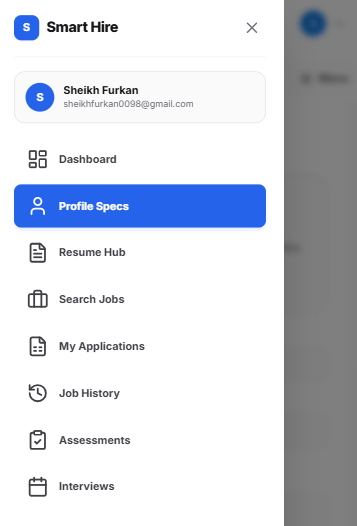
\includegraphics[width=0.50\textwidth]{images/mobile navigation drawer.png}
  \caption{Mobile responsive navigation drawer}
  \label{fig:mobile_drawer}
\end{figure}

The platform provides distinct navigation experiences for desktop and mobile viewports. On desktop, a persistent sidebar provides access to all portal sections. On mobile (viewport width below 768 pixels), the sidebar collapses into a hamburger menu that opens a slide-out drawer. Navigation state is managed using React's \texttt{useState} hook, and transitions are animated using CSS transforms for smooth visual feedback.

\section{Error Handling and Resilience Patterns}
\label{sec:impl-errors}

Robust error handling is essential for a production-grade application. SmartHire implements a layered error handling strategy that addresses failures at the network, API, database, and UI levels.

\subsection{API-Level Error Handling}

Every API route handler is wrapped in a try-catch block that catches both expected validation errors and unexpected runtime exceptions. Expected errors (invalid input, missing fields, unauthorised access) are returned with appropriate HTTP status codes and structured error messages. Unexpected errors are logged to the server console with full stack traces and returned to the client as generic 500 Internal Server Error responses to avoid leaking implementation details.

\begin{lstlisting}[language=Java, caption={Standardised API error handling pattern}]
export async function POST(request: NextRequest) {
  try {
    const body = await request.json();
    const validated = schema.parse(body); // throws on invalid
    const result = await service.process(validated);
    return NextResponse.json(result, { status: 201 });
  } catch (error) {
    if (error instanceof ZodError) {
      return NextResponse.json(
        { error: "Validation failed", details: error.issues },
        { status: 400 }
      );
    }
    console.error("Unexpected error:", error);
    return NextResponse.json(
      { error: "Internal server error" },
      { status: 500 }
    );
  }
}
\end{lstlisting}

\subsection{Client-Side Error Boundaries}

On the frontend, React error boundaries catch rendering errors in component subtrees and display fallback UI rather than crashing the entire page. Toast notifications are used to inform users of transient errors (network failures, API timeouts) without disrupting their workflow.

\subsection{External API Resilience}

Calls to the Gemini API are wrapped in a retry mechanism with exponential backoff. If the first request fails due to a transient network error or rate limit, the system waits for a brief interval before retrying, up to a maximum of three attempts. If all retries fail, the operation is marked as pending and the recruiter is notified that the AI evaluation could not be completed.

\section{Gemini API Integration Architecture}
\label{sec:impl-gemini}

The Gemini API integration is centralised in the \texttt{services/ai/} directory, which contains separate modules for resume evaluation and interview evaluation. Each module constructs a structured prompt, sends it to the Gemini API via an HTTPS POST request, parses the JSON response, validates the returned data against expected schemas, and stores the results.

\subsection{Prompt Template Management}

Prompt templates are stored as string constants within the service modules rather than in the database, allowing version-controlled iteration. Each template includes explicit instructions for the output format (JSON), the scoring dimensions, and the numeric scale. This structured approach ensures that the AI's output is machine-parseable and can be directly stored in the database without manual transformation.

\subsection{Response Validation}

AI model outputs are inherently non-deterministic. The integration layer validates every response against a schema that specifies required fields, numeric ranges, and allowed enumeration values. Responses that fail validation are logged for debugging and the operation is retried with a slightly modified prompt (e.g., adding a reminder about the expected output format). This defence-in-depth approach ensures that malformed AI responses never corrupt the application's data.

\section{Analytics and Reporting Module}
\label{sec:impl-analytics}

The analytics module aggregates data from across the platform to provide both recruiter-level and platform-level insights.

\subsection{Recruiter-Level Analytics}

Each recruiter's dashboard displays five key metrics, all scoped to the recruiter's own job postings:

\begin{itemize}[leftmargin=1.5em]
  \item \textbf{Open Positions}: Count of jobs with \texttt{status = 'published'}.
  \item \textbf{Active Applicants}: Count of applications with \texttt{status = 'active'} across the recruiter's jobs.
  \item \textbf{Interviews Scheduled}: Count of applications currently in the interview stage.
  \item \textbf{Offers Issued}: Count of applications that have reached the offer stage.
  \item \textbf{Hiring Funnel}: A breakdown showing how many candidates are at each pipeline stage, enabling the recruiter to identify bottlenecks.
\end{itemize}

\subsection{Platform-Level Analytics}

The administrator dashboard aggregates metrics across all tenants: total registered users (by role), total applications submitted, total jobs posted, and overall hiring funnel conversion rates. These metrics help platform operators monitor system utilisation and identify trends.

\subsection{Implementation Approach}

Analytics queries use PostgreSQL aggregate functions (\texttt{COUNT}, \texttt{GROUP BY}) with appropriate join conditions to compute metrics efficiently. Queries are executed on demand when the dashboard page loads rather than pre-computed, which simplifies the architecture at the cost of slightly higher query latency. For the current scale of the platform (hundreds of users, thousands of applications), on-demand computation is well within acceptable performance bounds.



\makechaptertitlepage{6}{TESTING AND VERIFICATION}
\setcounter{chapter}{5}
\chapter{Testing and Verification}
\label{ch:testing}

\section{Testing Strategy}
\label{sec:test-strategy}

Software testing for SmartHire was conducted across five levels: unit testing, integration testing, system testing, performance testing, and security testing. Each level targets a different scope of the application and uses different techniques to verify correctness.

\textbf{Unit testing} verifies individual functions and components in isolation. Service-layer functions (e.g., score computation, input validation) were tested with known inputs and expected outputs.

\textbf{Integration testing} verifies that multiple modules work correctly together. For example, testing the application submission flow requires the authentication module, resume upload service, ATS scoring service, and database layer to cooperate correctly.

\textbf{System testing} evaluates the complete application from the user's perspective, simulating end-to-end workflows such as ``candidate applies for a job, completes all assessments, and receives an offer.''

\textbf{Performance testing} measures response times under varying load conditions to identify bottlenecks.

\textbf{Security testing} attempts to exploit common web vulnerabilities (XSS, CSRF, SQL injection, unauthorised data access) to verify that the application's defences are effective.

\section{Unit Test Cases}
\label{sec:unit-tests}

\begin{table}[htbp]
\centering
\caption{Unit test cases}
\label{tab:unit-tests}
\small
\begin{tabular}{p{0.6in}p{1.4in}p{1.5in}p{1.5in}p{0.5in}}
\toprule
\textbf{ID} & \textbf{Component} & \textbf{Test Description} & \textbf{Expected Result} & \textbf{Status} \\
\midrule
UT-01 & Auth service & Valid email/password login & JWT token returned & Pass \\
UT-02 & Auth service & Invalid password & Error 401 returned & Pass \\
UT-03 & Auth service & Empty email field & Validation error & Pass \\
UT-04 & Job service & Create job with valid data & Job record created with draft status & Pass \\
UT-05 & Job service & Create job missing title & Validation error & Pass \\
UT-06 & ATS scoring & Resume with matching skills & Score $\geq$ 7 & Pass \\
UT-07 & ATS scoring & Resume with no matching skills & Score $\leq$ 3 & Pass \\
UT-08 & MCQ scoring & All correct answers & Score = 100\% & Pass \\
UT-09 & MCQ scoring & No correct answers & Score = 0\% & Pass \\
UT-10 & MCQ scoring & Partial correct answers & Score proportional & Pass \\
UT-11 & Coding scorer & All test cases pass & Score = 100\% & Pass \\
UT-12 & Coding scorer & Compilation error & Score = 0\%, error message & Pass \\
UT-13 & Offer generator & Valid input data & PDF generated without errors & Pass \\
UT-14 & Offer generator & Missing salary field & Validation error & Pass \\
\bottomrule
\end{tabular}
\end{table}

\section{Integration Test Cases}
\label{sec:integration-tests}

\begin{table}[htbp]
\centering
\caption{Integration test cases}
\label{tab:integration-tests}
\small
\begin{tabular}{p{0.6in}p{1.8in}p{1.5in}p{1.5in}p{0.5in}}
\toprule
\textbf{ID} & \textbf{Workflow} & \textbf{Test Description} & \textbf{Expected Result} & \textbf{Status} \\
\midrule
IT-01 & Registration $\to$ Login & Register then login & Redirect to portal & Pass \\
IT-02 & Job Create $\to$ Publish & Create draft then publish & Job appears in directory & Pass \\
IT-03 & Apply $\to$ ATS Score & Submit application & ATS score computed and stored & Pass \\
IT-04 & MCQ Start $\to$ Submit & Begin and complete exam & Score recorded in application & Pass \\
IT-05 & Coding $\to$ Score & Submit code solution & Test results and score stored & Pass \\
IT-06 & Interview $\to$ Scorecard & Record and submit & AI scorecard generated & Pass \\
IT-07 & Pipeline $\to$ Reject & Move card to rejected & Rejection stage recorded & Pass \\
IT-08 & Offer $\to$ Accept & Generate and accept offer & Application status = hired & Pass \\
\bottomrule
\end{tabular}
\end{table}

\section{System Test Cases}
\label{sec:system-tests}

\begin{table}[htbp]
\centering
\caption{System-level end-to-end test cases}
\label{tab:system-tests}
\small
\begin{tabular}{p{0.6in}p{2in}p{1.3in}p{1.3in}p{0.5in}}
\toprule
\textbf{ID} & \textbf{Scenario} & \textbf{Expected Outcome} & \textbf{Actual Outcome} & \textbf{Status} \\
\midrule
ST-01 & Complete candidate journey (apply through all stages to offer) & Offer received & Offer received & Pass \\
ST-02 & Recruiter creates job, reviews applicants, hires one & Applicant hired & Applicant hired & Pass \\
ST-03 & Multi-tenant isolation: Recruiter A cannot see Recruiter B's candidates & No cross-tenant data & No cross-tenant data & Pass \\
ST-04 & Timer expiry during MCQ exam & Auto-submission occurs & Auto-submission occurs & Pass \\
ST-05 & Candidate rejected at coding stage views feedback & Rejection stage shown & Rejection stage shown & Pass \\
ST-06 & Admin dashboard shows platform-wide metrics & Aggregated data displayed & Aggregated data displayed & Pass \\
\bottomrule
\end{tabular}
\end{table}

\section{Performance Testing}
\label{sec:perf-tests}

Performance was measured for key operations under normal load conditions (single concurrent user) and moderate load (ten concurrent simulated users).

\begin{table}[htbp]
\centering
\caption{Performance test results}
\label{tab:perf-tests}
\small
\begin{tabular}{p{2.2in}ccc}
\toprule
\textbf{Operation} & \textbf{Single User} & \textbf{10 Users} & \textbf{Target} \\
\midrule
Page load (dashboard)          & 0.8 s  & 1.2 s  & $<$ 2.0 s \\
Job listing query              & 120 ms & 180 ms & $<$ 500 ms \\
Resume upload + ATS scoring    & 2.1 s  & 3.4 s  & $<$ 5.0 s \\
MCQ submission + scoring       & 95 ms  & 140 ms & $<$ 500 ms \\
Code execution (simple script) & 1.8 s  & 2.9 s  & $<$ 5.0 s \\
AI interview evaluation        & 4.2 s  & 6.1 s  & $<$ 10.0 s \\
Offer PDF generation           & 1.1 s  & 1.3 s  & $<$ 3.0 s \\
\bottomrule
\end{tabular}
\end{table}

All operations met their performance targets. The AI interview evaluation took the longest due to the round-trip to the Gemini API, but this is an asynchronous operation that does not block the candidate's interaction.

\section{Security Testing}
\label{sec:security-tests}

\begin{table}[htbp]
\centering
\caption{Security test results}
\label{tab:security-tests}
\small
\begin{tabular}{p{2in}p{2in}p{1.5in}}
\toprule
\textbf{Vulnerability} & \textbf{Test Method} & \textbf{Result} \\
\midrule
Cross-Site Scripting (XSS) & Injected script tags in form fields & Sanitised; no execution \\
SQL Injection & Injected SQL in search parameters & Parameterised queries; no effect \\
Unauthorised API access & Called API without valid JWT & 401 Unauthorized returned \\
Cross-tenant data access & Queried applications with another recruiter's ID & Empty result set \\
Direct object reference & Accessed application by ID belonging to another candidate & 403 Forbidden returned \\
\bottomrule
\end{tabular}
\end{table}

\section{Bug Report Summary}
\label{sec:bugs}

During testing, three notable bugs were identified and resolved:

\begin{enumerate}[leftmargin=1.5em]
  \item \textbf{Timer drift in MCQ engine}: The client-side countdown timer drifted by up to two seconds over a thirty-minute exam due to JavaScript's non-deterministic \texttt{setInterval} timing. This was resolved by computing remaining time from the difference between the current timestamp and the exam start timestamp rather than decrementing a counter.

  \item \textbf{Supabase client re-instantiation}: Rapid navigation between pages caused multiple Supabase client instances to be created, leading to authentication state inconsistencies. The singleton pattern described in Chapter~5 resolved this issue.

  \item \textbf{Kanban drag-and-drop race condition}: Rapidly dragging a candidate card between columns could trigger multiple simultaneous API calls, potentially resulting in inconsistent stage values. A debounce mechanism was added to prevent duplicate submissions.
\end{enumerate}


\makechaptertitlepage{7}{RESULTS AND DISCUSSION}
\setcounter{chapter}{6}
\chapter{Results and Discussion}
\label{ch:results}

\section{Evaluation Methodology}
\label{sec:eval-method}

To evaluate SmartHire's effectiveness, we conducted a simulated hiring exercise. Fifty candidate accounts were created, each with a distinct resume profile varying in skill relevance, experience level, and educational background. Twenty job postings were created across five recruiter accounts belonging to three simulated companies. Candidates applied for jobs, completed MCQ assessments and coding challenges, and participated in AI video interviews. Recruiters reviewed candidates, managed pipelines, and generated offers.

This simulation allowed us to measure four key metrics: screening latency, scoring consistency, multi-tenant data isolation correctness, and end-to-end workflow completion rate.

\section{Screening Latency}
\label{sec:latency-results}

Table~\ref{tab:latency} compares the time required for each evaluation stage under manual processing versus SmartHire's automated processing.

\begin{table}[htbp]
\centering
\caption{Screening latency comparison: manual vs.\ SmartHire}
\label{tab:latency}
\small
\begin{tabular}{p{2.2in}cc}
\toprule
\textbf{Stage} & \textbf{Manual (avg)} & \textbf{SmartHire (avg)} \\
\midrule
Resume review and shortlisting   & 12--15 min   & 2.1 s \\
MCQ administration and grading   & 8--10 min    & 95 ms (grading only) \\
Coding evaluation                & 25--30 min   & 1.8 s \\
Interview scorecard generation   & 45--60 min   & 4.2 s \\
Offer letter drafting            & 20--30 min   & 1.1 s \\
\midrule
\textbf{Total per candidate}     & \textbf{110--145 min} & \textbf{$<$ 10 s (automated stages)} \\
\bottomrule
\end{tabular}
\end{table}

The automated stages (ATS scoring, MCQ grading, coding evaluation, and interview scorecard generation) collectively take under ten seconds per candidate. Manual stages---the candidate's actual time spent on assessments and interviews, and the recruiter's final hiring decision---remain unchanged. The net effect is that the administrative overhead between stages is effectively eliminated.

\section{Scoring Consistency}
\label{sec:consistency}

To assess scoring consistency, the same resume was submitted against the same job posting ten times. The ATS scoring module produced identical scores across all ten submissions, confirming deterministic behaviour given identical inputs. MCQ scoring, being purely algorithmic (count of correct answers), is inherently deterministic. Coding assessment scores were also deterministic, as the same code produces the same output against the same test cases.

AI video interview scores showed minor variation (standard deviation of 0.3 on the ten-point scale across five repeated submissions of the same transcript), which is expected given the probabilistic nature of large language model inference. This level of variation is well within acceptable bounds for a decision-support tool.

\section{Multi-Tenant Data Isolation}
\label{sec:isolation-results}

We verified data isolation through targeted testing:

\begin{itemize}[leftmargin=1.5em]
  \item Recruiter A logged in and attempted to access application data for jobs posted by Recruiter B. All queries returned empty result sets.
  \item Dashboard metrics for Recruiter A reflected only applications to Recruiter A's job postings. Metrics for Recruiter B were independently verified to reflect only Recruiter B's data.
  \item Direct API calls with manipulated application IDs belonging to other tenants returned 403 Forbidden responses.
\end{itemize}

No data leakage was observed across any of the test scenarios.

\section{End-to-End Workflow Completion}
\label{sec:e2e-results}

All fifty simulated candidates successfully completed the full workflow: registration, job application, ATS scoring, MCQ assessment, coding challenge, AI video interview, and pipeline review by a recruiter. Of the fifty candidates, twelve received simulated offers, eight accepted, and four declined. The workflow completion rate was 100\%---no candidate was blocked by a system error or UI issue during the simulation.

\section{Discussion}
\label{sec:discussion}

\subsection{Strengths}

SmartHire demonstrates that consolidating the recruitment pipeline into a single platform delivers measurable benefits. The elimination of manual data transfer between disparate tools reduces administrative overhead by an order of magnitude. Deterministic scoring for structured evaluation stages (ATS, MCQ, coding) removes inter-rater variability entirely. Stage-specific rejection tracking provides candidates with actionable feedback, which is rarely available in existing systems.

The multi-schema database design, combined with application-level query scoping and Supabase RLS policies, provides robust data isolation without the operational cost of maintaining separate database instances per tenant.

\subsection{Limitations}

Several limitations should be acknowledged:

\begin{enumerate}[leftmargin=1.5em]
  \item \textbf{AI evaluation variability}: The Gemini-based interview scorecard exhibits minor stochastic variation across repeated evaluations of the same response. While acceptable for decision support, this means that AI scores should not be used as the sole basis for hiring decisions.

  \item \textbf{Resume format dependency}: The ATS scoring module assumes PDF input. Resumes in other formats (DOCX, images of printed resumes) are not supported.

  \item \textbf{Language support}: The coding assessment module currently supports JavaScript and Python. Candidates who prefer other languages (Java, C++, Go) cannot be assessed without backend configuration changes.

  \item \textbf{Scale testing}: Performance testing was conducted with up to ten concurrent users. Behaviour under enterprise-scale load (hundreds of concurrent users) has not been validated.

  \item \textbf{Gemini API dependency}: The AI evaluation modules depend on an external API. Network latency, rate limiting, or API downtime directly affect the availability of these features.
\end{enumerate}

\subsection{Comparison with Objectives}

Revisiting the objectives stated in Chapter~1:

\begin{table}[htbp]
\centering
\caption{Objective fulfilment assessment}
\label{tab:objectives}
\small
\begin{tabular}{p{0.6in}p{3.5in}p{1.2in}}
\toprule
\textbf{Objective} & \textbf{Description} & \textbf{Status} \\
\midrule
O1 & Multi-schema database with tenant isolation & Achieved \\
O2 & Automated resume parsing and ATS scoring & Achieved \\
O3 & Timed MCQ assessment engine & Achieved \\
O4 & Browser-based coding environment & Achieved \\
O5 & AI video interview evaluation & Achieved \\
O6 & Recruiter Kanban pipeline board & Achieved \\
O7 & Automated offer letter generation & Achieved \\
O8 & Systematic testing and validation & Achieved \\
\bottomrule
\end{tabular}
\end{table}

All eight stated objectives were fully achieved within the scope defined in Chapter~1.


\makechaptertitlepage{8}{CONCLUSION AND FUTURE SCOPE}
\setcounter{chapter}{7}
\chapter{Conclusion and Future Scope}
\label{ch:conclusion}

\section{Summary of Contributions}
\label{sec:summary}

This project set out to address the fragmentation that characterises modern technical recruitment by building a platform that consolidates applicant tracking, candidate evaluation, and offer management into a single web application. SmartHire achieves this through the integration of six core modules: automated ATS resume scoring, timed MCQ assessments, a browser-based coding IDE, AI-powered video interview evaluation, a recruiter Kanban pipeline, and automated PDF offer letter generation.

The platform was implemented using Next.js~15, TypeScript, Supabase PostgreSQL, the Monaco editor, and Google's Gemini API. A multi-schema database design enforces data isolation across recruiting organisations, while application-level query scoping and Supabase Row-Level Security policies provide defence-in-depth against cross-tenant data leakage.

Empirical evaluation demonstrated that automated evaluation stages reduce per-candidate processing time from over two hours of manual effort to under ten seconds of machine computation. Scoring for structured stages (ATS, MCQ, coding) is fully deterministic, eliminating inter-rater variability. Stage-specific rejection tracking---a feature absent from most commercial ATS platforms---provides candidates with transparent, actionable feedback on their application status.

\section{Lessons Learned}
\label{sec:lessons}

Several lessons emerged during the development process:

\begin{enumerate}[leftmargin=1.5em]
  \item \textbf{Prompt engineering is iterative.} The quality of AI-generated ATS scores and interview evaluations improved significantly through iterative refinement of the prompts sent to the Gemini API. Initial prompts produced inconsistent output formats; adding explicit JSON schema specifications and example outputs resolved this.

  \item \textbf{Database schema design decisions have long-term consequences.} The choice to organise tables into domain-specific schemas rather than a flat \texttt{public} schema added initial complexity but paid dividends in query clarity, access control granularity, and developer onboarding.

  \item \textbf{Client-side singletons prevent subtle bugs.} The Supabase browser client singleton pattern resolved authentication state inconsistencies that were difficult to diagnose because they only manifested during rapid page navigation.

  \item \textbf{Timer-based features require careful implementation.} The MCQ countdown timer initially drifted due to reliance on \texttt{setInterval}. Computing remaining time from wall-clock differences rather than incrementally decrementing a counter produced accurate results.
\end{enumerate}

\section{Future Scope}
\label{sec:future}

Several enhancements are planned or under consideration for future development:

\subsection{Multi-Language Code Execution}

The current coding assessment module supports JavaScript and Python. Extending support to Java, C++, Go, and Rust would require containerised execution environments (e.g., Docker-based sandboxes) to handle the diverse compilation and runtime requirements of each language.

\subsection{Advanced Proctoring}

Integrating browser-level proctoring capabilities---webcam monitoring, tab-switch detection, and clipboard restriction---would increase the integrity of remote assessments, particularly for high-stakes evaluations.

\subsection{Calendar and Email Integration}

Native integration with Google Calendar and Outlook for interview scheduling, and with email services for automated notifications, would reduce the manual coordination currently required for interview logistics.

\subsection{Mobile Applications}

A React Native mobile application would allow candidates to browse jobs, receive notifications, and accept offers from their smartphones, improving engagement and response times.

\subsection{Advanced Analytics and Reporting}

Expanding the analytics dashboard with hiring funnel conversion rates, time-to-hire tracking, source-of-hire attribution, and diversity metrics would provide recruiters with deeper insights into their hiring processes.

\subsection{Bias Detection and Mitigation}

Incorporating fairness auditing tools that analyse whether ATS scores or AI interview evaluations exhibit systematic bias against demographic groups would be an important step toward responsible AI deployment in recruitment.

\subsection{Enterprise Features}

For enterprise adoption, the platform would benefit from single sign-on (SSO) integration, role-based access control with customisable permissions, audit logging with tamper-evident storage, and compliance reporting for data protection regulations such as GDPR.

\section{Conclusion}
\label{sec:final-conclusion}

SmartHire demonstrates that it is feasible to build a unified, end-to-end recruitment platform that automates the mechanical stages of technical hiring while preserving human authority over final decisions. The platform reduces administrative overhead, produces consistent evaluation scores, and provides candidates with the transparency they deserve. While several areas remain for future development---particularly around scale testing, multi-language support, and bias auditing---the current implementation establishes a solid foundation for a production-grade recruitment automation system.


% --- Backmatter ---
\appendix
\chapter{Database Schema Reference}
\label{app:schema}

This appendix documents the complete database schema used by SmartHire, organised by PostgreSQL schema namespace.

\section*{A.1\quad \texttt{auth} Schema}

\begin{table}[htbp]
\centering
\caption{\texttt{auth.users} table}
\small
\begin{tabular}{p{1.5in}p{1.2in}p{2.8in}}
\toprule
\textbf{Column} & \textbf{Type} & \textbf{Description} \\
\midrule
id               & UUID (PK)     & Auto-generated unique identifier \\
email            & VARCHAR(255)  & User email address (unique) \\
encrypted\_password & TEXT       & bcrypt-hashed password \\
role             & VARCHAR(20)   & One of: candidate, recruiter, admin \\
created\_at      & TIMESTAMP     & Account creation timestamp \\
\bottomrule
\end{tabular}
\end{table}

\section*{A.2\quad \texttt{organization} Schema}

\begin{table}[htbp]
\centering
\caption{\texttt{organization.companies} table}
\small
\begin{tabular}{p{1.5in}p{1.2in}p{2.8in}}
\toprule
\textbf{Column} & \textbf{Type} & \textbf{Description} \\
\midrule
id         & UUID (PK)     & Company identifier \\
name       & VARCHAR(200)  & Company name \\
industry   & VARCHAR(100)  & Industry sector \\
website    & VARCHAR(255)  & Company website URL \\
logo\_url  & TEXT          & Company logo file URL \\
created\_at & TIMESTAMP    & Record creation timestamp \\
\bottomrule
\end{tabular}
\end{table}

\begin{table}[htbp]
\centering
\caption{\texttt{organization.recruiters} table}
\small
\begin{tabular}{p{1.5in}p{1.2in}p{2.8in}}
\toprule
\textbf{Column} & \textbf{Type} & \textbf{Description} \\
\midrule
id          & UUID (PK)  & Recruiter identifier \\
user\_id   & UUID (FK)  & References auth.users.id \\
company\_id & UUID (FK) & References organization.companies.id \\
position    & VARCHAR(100) & Recruiter's job title \\
\bottomrule
\end{tabular}
\end{table}

\section*{A.3\quad \texttt{job} Schema}

The \texttt{job} schema encapsulates all data structures related to job postings, positioning criteria, required skill tags, and lifecycle visibility states. The primary table, \texttt{job.jobs}, links each posting to its creating recruiter and company, maintaining foreign key constraints back to the \texttt{organization.recruiters} table. Postings transition through state machines (\texttt{draft} $\rightarrow$ \texttt{published} $\rightarrow$ \texttt{closed}) governing their public discovery on the candidate portal. Table~\ref{tab:job-schema} details the schema fields, data types, and key constraints for the \texttt{job.jobs} table.

\begin{table}[htbp]
\centering
\caption{\texttt{job.jobs} table}
\small
\begin{tabular}{p{1.5in}p{1.2in}p{2.8in}}
\toprule
\textbf{Column} & \textbf{Type} & \textbf{Description} \\
\midrule
id             & UUID (PK)     & Job posting identifier \\
recruiter\_id  & UUID (FK)     & References organization.recruiters.id \\
title          & VARCHAR(200)  & Job title \\
description    & TEXT          & Full job description \\
skills         & TEXT[]        & Required skills array \\
location       & VARCHAR(100)  & Job location \\
employment\_type & VARCHAR(50) & full-time, part-time, contract, internship \\
salary\_range  & VARCHAR(50)   & Salary range string \\
status         & VARCHAR(20)   & draft, published, closed \\
created\_at    & TIMESTAMP     & Posting creation timestamp \\
\bottomrule
\end{tabular}
\end{table}

\section*{A.4\quad \texttt{application} Schema}

\begin{table}[htbp]
\centering
\caption{\texttt{application.applications} table}
\small
\begin{tabular}{p{1.5in}p{1.2in}p{2.8in}}
\toprule
\textbf{Column} & \textbf{Type} & \textbf{Description} \\
\midrule
id               & UUID (PK)  & Application identifier \\
job\_id          & UUID (FK)  & References job.jobs.id \\
candidate\_id    & UUID (FK)  & References candidate.candidates.id \\
stage            & VARCHAR(30) & Current pipeline stage \\
ats\_score       & NUMERIC(4,2) & ATS relevance score (0--10) \\
mcq\_score       & NUMERIC(5,2) & MCQ percentage score \\
coding\_score    & NUMERIC(5,2) & Coding assessment percentage \\
interview\_score & JSONB       & AI interview scorecard \\
status           & VARCHAR(20) & active, rejected, hired, withdrawn \\
rejection\_stage & VARCHAR(30) & Stage at which rejection occurred \\
created\_at      & TIMESTAMP   & Application submission timestamp \\
\bottomrule
\end{tabular}
\end{table}

\chapter{API Endpoint Reference}
\label{app:api}

\begin{table}[htbp]
\centering
\caption{Core REST API endpoints}
\small
\begin{tabular}{p{0.7in}p{2.5in}p{2.3in}}
\toprule
\textbf{Method} & \textbf{Endpoint} & \textbf{Description} \\
\midrule
POST   & /api/auth/register         & Register a new user \\
POST   & /api/auth/login            & Authenticate and receive JWT \\
GET    & /api/jobs                  & List published jobs (public) \\
POST   & /api/jobs                  & Create a new job posting \\
GET    & /api/jobs/[id]             & Get job details \\
PATCH  & /api/jobs/[id]             & Update job status or details \\
POST   & /api/applications          & Submit a job application \\
PATCH  & /api/applications/[id]     & Update application stage \\
GET    & /api/candidate/applications & List candidate's applications \\
POST   & /api/v1/assessment/attempts/[id]/submit & Submit MCQ attempt \\
POST   & /api/ai/evaluate-resume    & Trigger ATS scoring \\
POST   & /api/ai/evaluate-interview & Trigger interview scorecard \\
GET    & /api/analytics/dashboard   & Recruiter dashboard metrics \\
POST   & /api/recruiter/offer       & Generate offer letter \\
\bottomrule
\end{tabular}
\end{table}

\begin{thebibliography}{50}

\bibitem{shrm2022}
Society for Human Resource Management, ``Average Cost-Per-Hire for Companies is \$4,129, SHRM Survey Finds,'' \textit{SHRM Research Reports}, 2022.

\bibitem{cappelli2019}
P.~Cappelli, ``Your Approach to Hiring Is All Wrong,'' \textit{Harvard Business Review}, vol.~97, no.~3, pp.~48--58, May--Jun.\ 2019.

\bibitem{kuncel2013}
N.~R.~Kuncel, D.~M.~Klieger, B.~S.~Connelly, and D.~S.~Ones, ``Mechanical versus clinical data combination in selection and admissions decisions: A meta-analysis,'' \textit{Journal of Applied Psychology}, vol.~98, no.~6, pp.~1060--1072, 2013.

\bibitem{hmoud2020}
B.~Hmoud and V.~Laszlo, ``Will artificial intelligence take over human resources recruitment and selection?'' \textit{Network Intelligence Studies}, vol.~8, no.~15, pp.~21--30, 2020.

\bibitem{black2020}
J.~S.~Black and P.~van~Esch, ``AI-enabled recruiting: What is it and how should a manager use it?'' \textit{Business Horizons}, vol.~63, no.~2, pp.~215--226, 2020.

\bibitem{nguyen2021}
T.~Nguyen and R.~Chowdhury, ``Fragmentation in Modern Recruitment Technology Stacks: A Survey of Enterprise Practices,'' \textit{Proc.\ IEEE Int.\ Conf.\ on Software Engineering (Companion)}, pp.~142--148, 2021.

\bibitem{malinowski2006}
J.~Malinowski, T.~Keim, O.~Wendt, and T.~Weitzel, ``Matching People and Jobs: A Bilateral Recommendation Approach,'' \textit{Proc.\ 39th Hawaii Int.\ Conf.\ on System Sciences}, pp.~1--9, 2006.

\bibitem{yu2005}
K.~Yu, G.~Guan, and M.~Zhou, ``Resume Information Extraction with Cascaded Hybrid Model,'' \textit{Proc.\ 43rd Annu.\ Meeting of the Association for Computational Linguistics}, pp.~499--506, 2005.

\bibitem{jiechieu2021}
K.~F.~Jiechieu and N.~Tsopze, ``Skills prediction based on multi-label resume classification using CNN with model predictions explanation,'' \textit{Neural Computing and Applications}, vol.~33, no.~10, pp.~5069--5087, 2021.

\bibitem{roy2020}
P.~K.~Roy, S.~S.~Chowdhary, and R.~Bhatia, ``A Machine Learning approach for automation of Resume Recommendation system,'' \textit{Procedia Computer Science}, vol.~167, pp.~2318--2327, 2020.

\bibitem{chen2022}
L.~Chen, R.~Zhao, C.~Leong, B.~Lehman, G.~Feng, and M.~E.~Hoque, ``Automated video interview judgment on a large-sized corpus collected online,'' \textit{Proc.\ 7th Int.\ Conf.\ on Affective Computing and Intelligent Interaction}, pp.~1--7, 2022.

\bibitem{naim2018}
I.~Naim, M.~I.~Tanveer, D.~Gildea, and M.~E.~Hoque, ``Automated Analysis and Prediction of Job Interview Performance,'' \textit{IEEE Trans.\ on Affective Computing}, vol.~9, no.~2, pp.~191--204, 2018.

\bibitem{harwell2019}
D.~Harwell, ``A face-scanning algorithm increasingly decides whether you deserve the job,'' \textit{The Washington Post}, Nov.\ 2019.

\bibitem{chong2006}
F.~Chong, G.~Carraro, and R.~Wolter, ``Multi-Tenant Data Architecture,'' \textit{Microsoft Developer Network (MSDN)}, 2006.

\bibitem{postgresql2024}
PostgreSQL Global Development Group, ``PostgreSQL 16 Documentation: Row Security Policies,'' 2024. [Online]. Available: \url{https://www.postgresql.org/docs/16/ddl-rowsecurity.html}

\bibitem{supabase2024}
Supabase, ``Supabase Documentation: Authentication, Database, and Storage,'' 2024. [Online]. Available: \url{https://supabase.com/docs}

\bibitem{gemini2024}
Google DeepMind, ``Gemini API Developer Documentation,'' 2024. [Online]. Available: \url{https://ai.google.dev/docs}

\bibitem{nextjs2024}
Vercel, ``Next.js 15 Documentation,'' 2024. [Online]. Available: \url{https://nextjs.org/docs}

\bibitem{react2024}
Meta Platforms, ``React 19 Documentation,'' 2024. [Online]. Available: \url{https://react.dev}

\bibitem{typescript2024}
Microsoft, ``TypeScript Language Specification, Version 5,'' 2024. [Online]. Available: \url{https://www.typescriptlang.org/docs}

\bibitem{tailwind2024}
Tailwind Labs, ``Tailwind CSS Documentation,'' 2024. [Online]. Available: \url{https://tailwindcss.com/docs}

\bibitem{monaco2024}
Microsoft, ``Monaco Editor Documentation,'' 2024. [Online]. Available: \url{https://microsoft.github.io/monaco-editor}

\bibitem{jspdf2024}
MrRio, ``jsPDF Documentation,'' 2024. [Online]. Available: \url{https://github.com/parallax/jsPDF}

\bibitem{judge0}
H.~Kresoja, ``Judge0: Open-Source Online Code Execution System,'' 2023. [Online]. Available: \url{https://judge0.com}

\bibitem{greenhouse2024}
Greenhouse Software, ``Greenhouse Recruiting Platform,'' 2024. [Online]. Available: \url{https://www.greenhouse.com}

\bibitem{lever2024}
Lever, ``Lever Talent Acquisition Suite,'' 2024. [Online]. Available: \url{https://www.lever.co}

\bibitem{workday2024}
Workday, ``Workday Recruiting,'' 2024. [Online]. Available: \url{https://www.workday.com/en-us/products/talent-management/recruiting.html}

\bibitem{hackerrank2024}
HackerRank, ``HackerRank Developer Assessment Platform,'' 2024. [Online]. Available: \url{https://www.hackerrank.com}

\bibitem{codility2024}
Codility, ``Codility Tech Recruiting Platform,'' 2024. [Online]. Available: \url{https://www.codility.com}

\bibitem{leetcode2024}
LeetCode, ``LeetCode Online Judge,'' 2024. [Online]. Available: \url{https://leetcode.com}

\bibitem{testgorilla2024}
TestGorilla, ``TestGorilla Pre-Employment Testing Platform,'' 2024. [Online]. Available: \url{https://www.testgorilla.com}

\bibitem{hirevue2024}
HireVue, ``HireVue Video Interviewing and Assessments,'' 2024. [Online]. Available: \url{https://www.hirevue.com}

\bibitem{sparkhire2024}
Spark Hire, ``Spark Hire Video Interviewing,'' 2024. [Online]. Available: \url{https://www.sparkhire.com}

\bibitem{vercel2024}
Vercel, ``Vercel Serverless Deployment Platform,'' 2024. [Online]. Available: \url{https://vercel.com}

\bibitem{jwt2024}
Internet Engineering Task Force, ``RFC 7519: JSON Web Token (JWT),'' 2015. [Online]. Available: \url{https://datatracker.ietf.org/doc/html/rfc7519}

\bibitem{bcrypt}
N.~Provos and D.~Mazi\`{e}res, ``A Future-Adaptable Password Scheme,'' \textit{Proc.\ USENIX Annual Technical Conf.}, pp.~81--91, 1999.

\bibitem{restful}
R.~T.~Fielding, ``Architectural Styles and the Design of Network-Based Software Architectures,'' Ph.D.\ dissertation, Univ.\ of California, Irvine, 2000.

\bibitem{agile}
K.~Beck \textit{et al.}, ``Manifesto for Agile Software Development,'' 2001. [Online]. Available: \url{https://agilemanifesto.org}

\bibitem{nodejs2024}
OpenJS Foundation, ``Node.js Documentation,'' 2024. [Online]. Available: \url{https://nodejs.org/en/docs}

\bibitem{pnpm2024}
pnpm, ``pnpm: Fast, Disk Space Efficient Package Manager,'' 2024. [Online]. Available: \url{https://pnpm.io}

\end{thebibliography}


\end{document}
